%%%%%%%%%%%%%%%%%%%%%%%%%%%%%%%%%%%%%%%%%%%%%%%%%%%%%%%%%%%%%%%%%%%%%%%%%%%%%%
%%
%% This file is part of the Home2L project.
%%
%% (C) 2015-2018 Gundolf Kiefer
%%
%% Home2L is free software: you can redistribute it and/or modify
%% it under the terms of the GNU General Public License as published by
%% the Free Software Foundation, either version 3 of the License, or
%% (at your option) any later version.
%%
%% Home2L is distributed in the hope that it will be useful,
%% but WITHOUT ANY WARRANTY; without even the implied warranty of
%% MERCHANTABILITY or FITNESS FOR A PARTICULAR PURPOSE.  See the
%% GNU General Public License for more details.
%%
%% You should have received a copy of the GNU General Public License
%% along with Home2L. If not, see <https://www.gnu.org/licenses/>.
%%
%%%%%%%%%%%%%%%%%%%%%%%%%%%%%%%%%%%%%%%%%%%%%%%%%%%%%%%%%%%%%%%%%%%%%%%%%%%%%%



%%%%%%%%%%%%%%%%%%%%%%%%%%%%% General Header %%%%%%%%%%%%%%%%%%%%%%%%%%%%%%%%%


\documentclass[12pt,english,parskip=half]{scrreprt}
\usepackage[utf8]{inputenc}
\usepackage[a4paper,tmargin=15mm,bmargin=15mm,lmargin=20mm,rmargin=20mm,includehead,includefoot]{geometry}
\usepackage{lmodern}        % "Latin Modern" font allows italic+bold font
\usepackage[T1]{fontenc}    % see https://tex.stackexchange.com/questions/2369/why-do-the-less-than-symbol-and-the-greater-than-symbol-appear-wrong-as
\usepackage{amssymb}        % for the tutorial $\blacktriangleright$
\usepackage{longtable}
\usepackage{textcomp}       % for \textdegree
\usepackage{color}
\usepackage{paralist}       % for \begin{itemize}[...]

\usepackage{graphicx}

\usepackage{makeidx}       % for index
\usepackage[colorlinks=true,linkcolor=blue]{hyperref}    % clickable TOC and references with PDFlatex

\usepackage{listings}
\usepackage{lstautogobble}

%\usepackage[fencedCode=true]{markdown}   % for temporary use



\makeindex





%%%%%%%%%%%%%%%%%%%%%%%%%%%%% Settings %%%%%%%%%%%%%%%%%%%%%%%%%%%%%%%%%%%%%%%%


% Modes...
\ifdefined\version                         % 'public' version, for publishing ...
  \newcommand{\figfile}[2]{#2}             %   Omit references to image file
\else                                      % Working version ...
  \newcommand{\version}{Draft}
  \newcommand{\figfile}[2]{\href{#1}{#2}}  %   Create references to image files
\fi



% Project URL for links into the API docs. We probably can keep this empty to
% get relative links. With a browser like chromium with an integrated PDF
% viewer this should work, even if the PDF comes from a remote site.
% For locally stored documents, this is no problem anyway.

\newcommand{\projecturl}{}
%\newcommand{\projecturl}{https://github.com/gkiefer/home2l/}





%%%%%%%%%%%%%%%%%%% Headings, footers and formatting %%%%%%%%%%%%%%%%%%%%%%%%%%


\usepackage[headsepline,footsepline,plainfootsepline]{scrlayer-scrpage}
\pagestyle{scrheadings}

% Font settings...
\renewcommand{\familydefault}{\sfdefault}
\setkomafont{pageheadfoot}{\textsf}

\automark[chapter]{chapter}

\lohead{\headmark}
\cohead{}
\rohead{
\includegraphics[height=1.2em,keepaspectratio]{figs/home2l-icon}}

\lofoot*{\parbox[c][1.4em]{5cm}{The \emph{Home2L} Book}}
\cofoot*{} % \today}
\rofoot*{\thepage}
\renewcommand{\caplabelfont}{\textbf}





%%%%%%%%%%%%%%%%%%%%%%%%%%%%% Listings %%%%%%%%%%%%%%%%%%%%%%%%%%%%%%%%%%%%%%%%


\definecolor{lstbackground}{rgb}{0.9,0.9,0.9}

\lstloadlanguages{bash,C,C++,Python,VHDL}
\lstset{
  basicstyle=\ttfamily\footnotesize,
  keywordstyle=\bfseries,
  identifierstyle=,% nothing happens
  commentstyle=\color[rgb]{0.35,0.35,0.35},%\itshape
  backgroundcolor=\color{lstbackground},
  frame=single, %L, % single
  framerule=0pt,
  framesep=5pt,
  xleftmargin=5pt,
  xrightmargin=5pt,
  breaklines=true,
  postbreak=\mbox{\textcolor{red}{$\hookrightarrow$}},  % \space
  prebreak=\mbox{\textcolor{red}{$\hookleftarrow$}},
  autogobble=true,
  columns=fullflexible,  % to make copy-and-paste from the document work
  keepspaces=true,
  showstringspaces=false,
  language={}
}

\newcommand{\lst}[1]{\colorbox{lstbackground}{\ttfamily\footnotesize#1}}

\newcommand{\lstbox}[1]{
  \par
  \colorbox{lstbackground}{\ttfamily\footnotesize{\parbox{\linewidth}{#1}}}
  \par
}

%\renewcommand{\lstlistingname}{Listing}





%%%%%%%%%%%%%%%%%%%%%%%%%%%%%%% Info boxes %%%%%%%%%%%%%%%%%%%%%%%%%%%%%%%%%%%%


\newcommand{\infobox}[1]{
  \hfill
  \setlength\arrayrulewidth{1pt}
  \begin{tabular}[t]{c|c|}
    \parbox{1.8em}{\hfill\textit{\Huge\textbf{i}\,}}
    &
    \,\parbox{0.89\linewidth}{\setlength{\parskip}{0.5em}#1}\,
  \end{tabular}
  \par
}


\newcommand{\warnbox}[1]{
  \hfill
  \setlength\arrayrulewidth{1pt}
  \begin{tabular}[b]{c|c|}
    \includegraphics[width=1.8em,keepaspectratio]{figs/ic-warning}   %%% eps: inkscape -z -D -T $BASE.svg -E $BASE.eps
    &
    \,\parbox{0.89\linewidth}{\setlength{\parskip}{0.5em}#1}\,
  \end{tabular}
  \par
}





%%%%%%%%%%%%%%%%%%%%%%%%%%%%% Cross-referencing %%%%%%%%%%%%%%%%%%%%%%%%%%%%%%%


\newcommand{\toollabel}[1]{\index{#1@\texttt{#1} (tool)} \label{tool:#1}}
% similar labellings for RCs and ENVs are implicitly generated in 'excode.py'.
\newcommand{\envlabel}[1]{\index{#1@\texttt{#1} (configuration)} \label{env:#1}}
\newcommand{\rclabel}[2]{\index{#1@\texttt{#1} (resource driver)!#2@\texttt{#2} (resource)} \label{rc:#2}}

\newcommand{\idx}[1]{#1\index{#1}}

\newcommand{\envref}[1]{\hyperref[env:#1]{\texttt{#1}}}        % add index? last #1 -> '\idx{#1}'
\newcommand{\rcref}[1]{\hyperref[rc:#1]{\texttt{#1}}}
\newcommand{\toolref}[1]{\hyperref[tool:#1]{\texttt{\idx{#1}}}}

\newcommand{\docref}[2]{\href{\projecturl#1}{#2}}

\newcommand{\refapipython}{\docref{home2l-api_python/index.html}{Python API}}
\newcommand{\refapic}{\docref{home2l-api_c/index.html}{C/C++ API}}





%%%%%%%%%%%%%%%%%%%%%%%%%%%%%%%%%%%%%%%%%%%%%%%%%%%%%%%%%%%%%%%%%%%%%%%%%%%%%%%
%
%                  Front Matter
%
%%%%%%%%%%%%%%%%%%%%%%%%%%%%%%%%%%%%%%%%%%%%%%%%%%%%%%%%%%%%%%%%%%%%%%%%%%%%%%%


\begin{document}

\sloppy

%\pagenumbering{roman}

\begin{titlepage}
  \centering
  \vfill

  \figfile{figs/home2l-icon.svg}{
    
\includegraphics[width=5cm,keepaspectratio]{figs/home2l-icon}   %%% eps: inkscape -z -D -T $BASE.svg -E $BASE.eps
  }
  \vfill

  \scalebox{2.0} {\Huge \textsf{\textbf{The \emph{Home2L} Book}} } \\
  \vskip 2em
  \huge \textsf{\textbf{Clever Tools for a Private Smart Home}}
  \vfill

  \textsf{Gundolf~Kiefer}
  \vfill

  \LARGE Version: \version \\ ~ \\ \today
  \vfill

  \framebox{
    \parbox{3cm}{
      
\includegraphics[width=3cm,keepaspectratio]{figs/cc-by-sa}   %%% eps: inkscape -z -D -T $BASE.svg -E $BASE.eps
    }
    ~
    \parbox{12cm}{\footnotesize This work is licensed under the Creative Commons Attribution-ShareAlike 4.0 International License. To view a copy of this license, visit \url{http://creativecommons.org/licenses/by-sa/4.0/} or send a letter to Creative Commons, PO Box 1866, Mountain View, CA 94042, USA.}
  }
\end{titlepage}


\setcounter{secnumdepth}{3}
\setcounter{tocdepth}{3}

\tableofcontents

%\newpage
%\pagenumbering{arabic}




%%%%%%%%%%%%%%%%%%%%%%%%%%%%% Main chapters %%%%%%%%%%%%%%%%%%%%%%%%%%%%%%%%%%


%\part{Overview, Tools and Concepts}



%%%%%%%%%%%%%%%%%%%%%%%%%%%%%%%%%%%%%%%%%%%%%%%%%%%%%%%%%%%%%%%%%%%%%%%%%%%%%%%
%
%
\chapter{Introduction}
\label{ch:intro}
%
%
%%%%%%%%%%%%%%%%%%%%%%%%%%%%%%%%%%%%%%%%%%%%%%%%%%%%%%%%%%%%%%%%%%%%%%%%%%%%%%%



%%%%%%%%%%%%%%%%%%%%%%%%%%%%%%%%%%%%%%%%%%%%%%%%%%%%%%%%%%%%%%%%%%%%%%%%%%
\section{What Are the \emph{Home2Ls}?}
\label{sec:intro-overview}
%%%%%%%%%%%%%%%%%%%%%%%%%%%%%%%%%%%%%%%%%%%%%%%%%%%%%%%%%%%%%%%%%%%%%%%%%%


The \emph{Home2L} \texttt{[houmtu:l]} suite is a framework, library and set of tools
for automation in private smart homes. Its main features and design goals are:


\subsection*{Efficient and Lightweight Design}

All core components are written in C/C++, with a very minimum set of external
dependencies beyond \texttt{libc} - ideally suited for small embedded devices and
microcontrollers. There is no need for a Java runtime environment or heavy web
frameworks. Starting up a server and command shell and shutting them down again
takes less than one second altogether - on an ARM-based minicomputer running
at 144 MHz!


\subsection*{Ambient Intelligence, No Need for a Central Server}

Central servers are single points of failure. \emph{Home2L} follows a completely
distributed concept. Any (mini-)computer can act as part of the network. If
resources, such as sensors or actors, are connected to them, they can be
exported to any other host in the \emph{Home2L} network. A failure of a host only
causes its own resources to be unavailable - everything else keeps on working.


\subsection*{Automation Rules Written in Python - But not Limited to That}

There is no new language or tool to learn to formulate automation rules.
\emph{Home2L} rules are typically formulated in Python, they profit from the
both the simplicity and the power of the Python language.
There can be multiple rules scripts, they may run on any machine, and
they may by combined with other software routines.

Other ways to interact with \emph{Home2L} resources is via the C/C++ API from any
application or by shell scripts using the \emph{Home2L Shell} in non-interactive mode.


\subsection*{Easy Driver Development in C/C++, Python or Any Other Language}

An API for \emph{resource} drivers allows to easily add support for new hardware.
A driver can be implemented

- in native C/C++ code (e.g. \emph{GPIO}).
- as a shell script (e.g. \emph{Weather}).
- in Python (examples can be found in the tutorial).


\subsection*{Privacy}

The \emph{Home2Ls} do not need any Internet connection and do not try to communicate
with hosts other than they are configured to. By design, the \emph{Home2Ls}
communicate with each other over a (trusted) LAN, which can easily be set up
and secured using standard Linux/UNIX techniques. The open source licensing ensures
transparency for what the software does inside the user's private home.


\subsection*{Modularity}

The core part, the \emph{Resources} library, is kept small and portable with APIs
for application programs \emph{and} drivers in C/C++ and Python. All other components
are optional and can be used or replaced by alternatives as desired by the user.

Figure~\ref{fig:home2l-components} shows an overview on the \emph{Home2L} components.

\begin{figure}[ht]
  \centering
  \figfile{figs/home2l-components.svg}{
    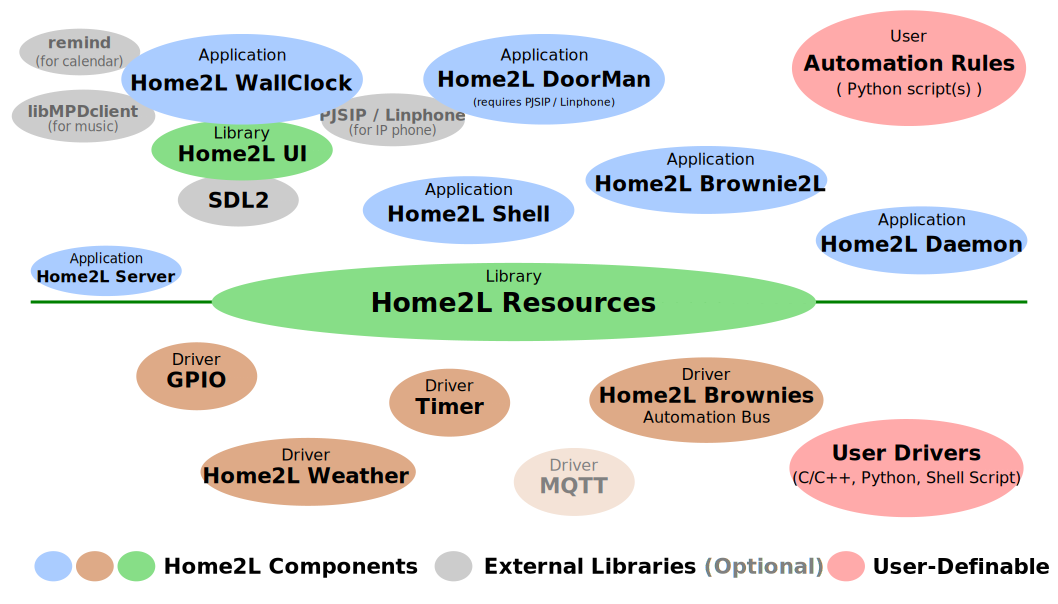
\includegraphics[width=0.9\linewidth,keepaspectratio]{figs/home2l-components}   %%% eps: inkscape -z -D -T $BASE.svg -E $BASE.eps
  }
  \caption[l]{\emph{Home2L} Components:
    \textcolor[rgb]{0.2,0.3,1.0}{Tools},
    \textcolor[rgb]{0.5,0.25,0}{Drivers},
    \textcolor[rgb]{0,0.5,0}{Libraries}
  }
  \label{fig:home2l-components}
\end{figure}




%%%%%%%%%%%%%%%%%%%%%%%%%%%%%%%%%%%%%%%%%%%%%%%%%%%%%%%%%%%%%%%%%%%%%%%%%%
\section{About This Book}
\label{sec:intro-about}
%%%%%%%%%%%%%%%%%%%%%%%%%%%%%%%%%%%%%%%%%%%%%%%%%%%%%%%%%%%%%%%%%%%%%%%%%%

This book serves as the central user and reference manual for the \emph{Home2L} suite.

Further information can be found in the \refapic{} and the \refapipython{} documentation.
Consulting the API documentation is particularly helpful for writing own resource drivers,
sophisticated automation rules or applications using some \emph{Home2L} library.

Presently, the \textit{Home2L Book} is still under construction and primarily targets readers with computer skills. Not all existing features are already documented in this book.
Extending the book to provide good end-user documentation is subject to future work
(see Section~\ref{sec:helping}).

Chapter~\ref{ch:tutorial} contains a step-by-step tutorial covering the installation,
concepts and all core tools of the suite. This should be the starting point for any new user.

Chapters~\ref{ch:installing} and ~\ref{ch:managing} describe the installation and management
of an installation, respectively. Chapter~\ref{ch:resources} explains the concepts and usage
of the \emph{Resources} library, the core component of the \emph{Home2L} suite.
This is followed by instructions on writing automation rules (Chapter~\ref{ch:rules}) and
drivers (Chapter~\ref{ch:drvdev}).
Chapter~\ref{ch:drvlib} documents the drivers contained in the \emph{Home2L} base distribution.
The remaining chapters cover the main user applications, presently
the \emph{Home2L WallClock} (Chapter~\ref{ch:wallclock}) and
the \emph{Home2L DoorMan} (Chapter~\ref{ch:doorman}).





%%%%%%%%%%%%%%%%%%%%%%%%%%%%%%%%%%%%%%%%%%%%%%%%%%%%%%%%%%%%%%%%%%%%%%%%%%
\section{How Can I Help?}
\label{sec:helping}
%%%%%%%%%%%%%%%%%%%%%%%%%%%%%%%%%%%%%%%%%%%%%%%%%%%%%%%%%%%%%%%%%%%%%%%%%%


Until now, the \emph{Home2L}  project has been developed by a single private person
in his spare time. The code has been published with the hope that is useful to
the community.

To let the project grow further and make available to a wider audience,
volunteers are needed and welcome.

Great contributions for the community would be, for example:

\begin{enumerate}
  \item Make \textbf{sample installations} and document them.

  \item \textbf{Packaging}: Create packages for major Linux distributions.

  \item \textbf{Documentation}: Write good documentation, particularly for end users.

  \item \textbf{Drivers:} Implement drivers for any hardware you like or have.
    Help with an \emph{MQTT} bridge would be appreciated, too.

  \item \textbf{Bridges to other home automation frameworks:} Implement drivers to interface
    with other open home automation frameworks.

  \item \textbf{Report and help fixing bugs.}

  \item \textbf{Translations} and internationalization.

  \item Write an \textbf{HTML frontend}.
\end{enumerate}

For any questions on how to participate, do not hesitate to contact the author
via the project page.





%%%%%%%%%%%%%%%%%%%%%%%%%%%%%%%%%%%%%%%%%%%%%%%%%%%%%%%%%%%%%%%%%%%%%%%%%%%%%%%
%
%
\chapter{Tutorial: Have a Test Drive!}
\label{ch:tutorial}
%
%
%%%%%%%%%%%%%%%%%%%%%%%%%%%%%%%%%%%%%%%%%%%%%%%%%%%%%%%%%%%%%%%%%%%%%%%%%%%%%%%

%\lstset{language=bash}



%%%%%%%%%%%%%%%%%%%%%%%%%%%%%%%%%%%%%%%%%%%%%%%%%%%%%%%%%%%%%%%%%%%%%%%%%%
\section{Introduction}
\label{sec:tutorial-intro}
%%%%%%%%%%%%%%%%%%%%%%%%%%%%%%%%%%%%%%%%%%%%%%%%%%%%%%%%%%%%%%%%%%%%%%%%%%


\subsection{Overview}

This step-by-step tutorial aims to give an exhaustive introduction to the
\emph{Home2L} suite covering the installation and all core tools and concepts of the suite.
It should be the starting point for anybody new to the software.

During the tutorial, you will

\begin{itemize}
  \item compile and install the \emph{Home2L} suite.

  \item learn about the \emph{Home2L} concepts: distributed and modular design,
    \emph{Home2L Resources}, tools, drivers, automation rules.

  \item learn about \emph{Home2L Resources}:
    values and states, subscriptions, requests, the directory.

  \item use the \emph{Home2L Shell} for inspection, maintenance, and logging.

  \item get acquainted with several tools: \toolref{home2l-shell},
    \toolref{home2l-wallclock}, \toolref{home2l-daemon}, \toolref{home2l-server}.

  \item explore the \emph{WallClock} (including the music player and calendar).

  \item learn how to write automation rules.

  \item obtain and understand a sample installation, which can be the starting point for
    your own home installation.

  \item get references to further information.

\end{itemize}

The tutorial is carried out on a virtual machine (VM) running Debian Linux, which will
be created as the first step. This just takes very few minutes and makes the \emph{Home2L}
installation process fully transparent, since no pre-configured boot image is necessary.

Sections \ref{sec:tutorial-vm} - \ref{sec:tutorial-install} deal with the installation.
Section~\ref{sec:tutorial-firststeps} will guide you through the \emph{ShowHouse},
a virtual example \emph{Home2L} installation. Section~\ref{sec:tutorial-shell} introduces the Nhome2L
Shell together with the basic concepts about Home2L resources.
The remaining subsections cover dedicated topics and can be exercised independent
from each other, depending on your interests and preferences.



\subsection{Notational Conventions}

The tutorial uses the following conventions in notation:

\begin{enumerate}[a)]
  \item A black triangle ($\blacktriangleright$) marks an instruction to follow.
  \item \lst{Typewriter text with a grey background} marks an interaction with your computer.
    Lines starting with a prompt indicate commands to be entered into the respective
    interpreter:
    \begin{description}
      \item[\lst{\$}] -- the Linux shell (\texttt{bash}),
      \item[\lst{home2l\textgreater}] -- the \emph{Home2L Shell},
      \item[\lst{\textgreater\textgreater\textgreater}] --the Python command interpreter.
    \end{description}
  \item Blocks with a big italic '\textbf{\textit{i}}' provide additional information.
\end{enumerate}

\textbf{Example:}

\begin{itemize}[$\blacktriangleright$]
  \item Enter the following commands to verify your computer's calculation skills:
    \begin{lstlisting}
    $ python3
    >>> 2+3
    5
    \end{lstlisting}
    Then push \emph{Ctrl-D} to quit the Python shell again.
\end{itemize}

\infobox{
  This is some additional information, not essential to just run the tutorial successfully.
}





%%%%%%%%%%%%%%%%%%%%%%%%%%%%%%%%%%%%%%%%%%%%%%%%%%%%%%%%%%%%%%%%%%%%%%%%%%
\section{Setting up a Virtual Machine}
\label{sec:tutorial-vm}
%%%%%%%%%%%%%%%%%%%%%%%%%%%%%%%%%%%%%%%%%%%%%%%%%%%%%%%%%%%%%%%%%%%%%%%%%%


\emph{Estimated Time: 45 Minutes (in large parts unattended)}


\infobox{
  If you already have a machine (physical or virtual) running Debian Linux
  or some derivative (other distributions should work as well, but has not been tested),
  you can skip the VM creation and continue with Section~\ref{sec:tutorial-prerequisites}
  on your existing machine -- at your choice.
}



%%%%%%%%%%%%%%%%%%%%%%%%%%%%%%%%%%%%%%%%%%%%%%%%%%%%%%%%%%%%
\subsection{System Requirements}
\label{sec:tutorial-vm-requirements}
%%%%%%%%%%%%%%%%%%%%%%%%%%%%%%%%%%%%%%%%%%%%%%%%%%%%%%%%%%%%


The following instructions have been tested with \textit{VirtualBox 5.2.10} and a
\textit{Debian 9.6 (Stretch)} guest system.

Up to 16 GB of disk space and 512 MB RAM will be needed for the virtual machine.

\infobox{
  The VM installations steps are \emph{much} faster if the VM
  is stored on RAM disk or an SSD instead of a mechanical hard disk.
}



%%%%%%%%%%%%%%%%%%%%%%%%%%%%%%%%%%%%%%%%%%%%%%%%%%%%%%%%%%%%
\subsection{Creating the VM and Preparing the Installation Medium}
\label{sec:tutorial-vm-create}
%%%%%%%%%%%%%%%%%%%%%%%%%%%%%%%%%%%%%%%%%%%%%%%%%%%%%%%%%%%%


\infobox{
  The following steps mention Linux/Unix shell commands for illustration purposes.
  Of course, any OS capable of running \textit{VirtualBox} can be used.
  Please use the respective (graphical) tools of your OS to download, unpack and
  run the virtual machine.
}


\begin{itemize}[$\blacktriangleright$]
\item
  Create an empty working directory 'home2l-tutorial' and change into it:

  \begin{lstlisting}[language=bash]
    $ mkdir home2l-tutorial
    $ cd home2l-tutorial
  \end{lstlisting}

\item
  Download and unpack the virtual machine:

  \begin{lstlisting}[language=bash]
    $ wget https://github.com/gkiefer/home2l/raw/master/home2l-showcase.tar.gz
        # or copy that file from a <home2l source>/home2l-showcase.tar.gz
    $ tar xzf home2l-showcase.tar.gz
  \end{lstlisting}

\item
  Download and provide a Debian installation image as 'install.iso' in the same directory:

  \begin{lstlisting}[language=bash]
    $ wget https://cdimage.debian.org/debian-cd/current/i386/iso-cd/debian-9.6.0-i386-netinst.iso
        # Adapt the path as necessary. We need an i386 "netinst" image.
        # More information can be found on the Debian download page at
        # https://cdimage.debian.org.
    $ ln -s debian-*.iso install.iso
        # or rename the file (if your OS does not support symbolic links)
  \end{lstlisting}

  The virtual machine comes with an empty harddisk image and is configured
  to have the CD/DVD image \texttt{'install.iso'} inserted in its optical drive.

\item
  Start \textit{VirtualBox}, select ''Machine $\rightarrow$ Add...'' and navigate to
  \begin{lstlisting}
  home2l-showcase/home2l-showcase.vbox
  \end{lstlisting}
  to add the \textit{Home2L ShowCase VM} as new virtual machine.
\end{itemize}



%%%%%%%%%%%%%%%%%%%%%%%%%%%%%%%%%%%%%%%%%%%%%%%%%%%%%%%%%%%%
\subsection{Installing Debian Linux}
\label{sec:tutorial-vm-debian}
%%%%%%%%%%%%%%%%%%%%%%%%%%%%%%%%%%%%%%%%%%%%%%%%%%%%%%%%%%%%


\begin{itemize}[$\blacktriangleright$]

\item
  Start the virtual machine -- either using the graphical UI of $VirtualBox$ or by running the
  following command on the command line:

  \begin{lstlisting}
  $ virtualbox --startvm home2l-showcase
  \end{lstlisting}

  The VM automatically boots from the Debian installation medium and runs the installer.

\item
  During the installation, \emph{accept all default settings or leave fields empty},
  except for the following options:

  \begin{enumerate}
    \item Select your country, language and keyboard layout as convenient for you.
    \item As a computer name, enter: \lst{home2l-showcase}.
    \item Leave the root password empty (will allow \texttt{home2l} to use \texttt{sudo} for root access).
    \item As the name for the first normal user enter: \lst{home2l}
    \item For user '\texttt{home2l}' enter a password at your choice (and do not forget it!).
    \item In the hard disk partitioning dialog you can accept all defaults. Only in the last step, you need to
      explicitly select ''yes'' to write the partition table to disk.

      \emph{The installer now requires approx. 5 minutes (or $<1$ minute when using a RAM disk.)
        without interaction to install the base system.}

    \item In the software selection dialog (aka ''\texttt{tasksel}''), select ''\lst{Xfce}'' and the
      \lst{standard system utilities} (the latter may appear translated to your language) and
      \emph{uncheck everything else}.

      \emph{The installer now requires approx. 30 minutes  (or 10 minutes when using a RAM disk.)
        without interaction (depending on your internet bandwidth and hard disk model).}

    \item Install the GRUB bootloader to \lst{/dev/sda}.
  \end{enumerate}

\item
  Finally, confirm to reboot the system.

  The installation medium is ''ejected'' automatically, the system reboots and you can log in as user
  \texttt{home2l} and use the system.

\end{itemize}



%%%%%%%%%%%%%%%%%%%%%%%%%%%%%%%%%%%%%%%%%%%%%%%%%%%%%%%%%%%%
\subsection{Logging in to the Virtual Machine}
\label{sec:tutorial-vm-login}
%%%%%%%%%%%%%%%%%%%%%%%%%%%%%%%%%%%%%%%%%%%%%%%%%%%%%%%%%%%%


You should now open this book inside the virtual machine.
This will allow you to copy and paste terminal commands from this document into the terminal
by marking with the left mouse button and pasting with the middle button.


\begin{itemize}[$\blacktriangleright$]

\item
  Log in as user \texttt{home2l} and start a terminal window.

\item
  Get the \emph{Home2L} source tree:
  \begin{lstlisting}[language=bash]
    $ sudo apt install git    # install git
    $ git clone https://github.com/gkiefer/home2l.git
  \end{lstlisting}

\item
  Open the \emph{Home2L Book}:
  \begin{lstlisting}
    $ evince ~/home2l/home2l-book.pdf &
  \end{lstlisting}
  Navigate to the tutorial section, page~\thepage.

\end{itemize}



%%%%%%%%%%%%%%%%%%%%%%%%%%%%%%%%%%%%%%%%%%%%%%%%%%%%%%%%%%%%
\subsection{Finalizing the Virtual Machine}
\label{sec:tutorial-vm-guestadditions}
%%%%%%%%%%%%%%%%%%%%%%%%%%%%%%%%%%%%%%%%%%%%%%%%%%%%%%%%%%%%

For optimum experience, the guest display should have at least 1600x900 pixels.
To allow such a resolution, the \emph{Virtual Box Guest Additions} must be installed in the VM.

\begin{itemize}[$\blacktriangleright$]

\item
  Add the \emph{Debian backports} repository to \texttt{etc/apt/sources.list}:
  \begin{lstlisting}
  $ echo -e "\n\n# Debian backports" \
      "\ndeb http://ftp.debian.org/debian stretch-backports main contrib non-free" \
      | sudo tee -a /etc/apt/sources.list
  \end{lstlisting}

\item
  Update the \texttt{apt} databas und install pending security and other updates:
  \begin{lstlisting}[language=bash]
    $ sudo apt -y purge pulseaudio   # pulseaudio has no use here and may cause problems
    $ sudo apt update
    $ sudo apt upgrade
  \end{lstlisting}

\item
  Then install the guest additions:
  \begin{lstlisting}[language=bash]
    $ sudo apt install linux-headers-686   # This must be installed before!
    $ sudo apt install virtualbox-guest-source virtualbox-guest-dkms \
        virtualbox-guest-utils
  \end{lstlisting}

\item
  Maximize your \emph{VirtualBox} window and reboot the VM to activate the guest additions.
  Then make sure that the \emph{''Auto-resize Guest Display''} option is on in \emph{VirtualBox}
  and login again.

  If the VM's desktop does not auto-resize properly to fill the window, you may either
  reboot once more or try to run:
  \begin{lstlisting}
    $ xrandr --output VGA-1 --preferred
  \end{lstlisting}
  (Run \texttt{xrandr} without parameters to list the exact name of the output and available resolutions.)

\end{itemize}


\begin{center}
\textbf{Your done -- Your VM is ready for the \emph{Home2L} installation!}
\end{center}


\infobox{
  \begin{enumerate}

  \item
    The \emph{VirtualBox Guest Additions} are \emph{only} required for optimizing the screen
    resolution of the VM. If their installation fails, you can continue without them.
    In this case, you should move the PDF viewer to a second virtual desktop in the VM.
    Without it on the main desktop, a resolution of 1024x768 pixels is sufficient to run the tutorial.

  \item
    The VM has been pre-configured to use ''NAT'' networking. This is the most fail-safe setting and
    allows the VM to share the internet connection with your host. If you want to contact the VM from
    your host or some other machine in your LAN, you may change the network setting to ''bridged''.
    Please consult the \textit{VirtualBox} documentation for details.

  \end{enumerate}
}





%%%%%%%%%%%%%%%%%%%%%%%%%%%%%%%%%%%%%%%%%%%%%%%%%%%%%%%%%%%%%%%%%%%%%%%%%%
\section{Installing Prerequisites}
\label{sec:tutorial-prerequisites}
%%%%%%%%%%%%%%%%%%%%%%%%%%%%%%%%%%%%%%%%%%%%%%%%%%%%%%%%%%%%%%%%%%%%%%%%%%


\emph{Estimated Time: 5 Minutes}


\begin{itemize}[$\blacktriangleright$]

\item
  If not done yet: Log in as user \texttt{home2l}, start a terminal window,
  and open this book inside the VM as described in Section~\ref{sec:tutorial-vm-login}.

\item
  Install all required packages for building and running the tutorial:
  \begin{lstlisting}
    $ sudo apt install make g++ \
        python3 python3-dev swig libreadline-dev curl \
        libsdl2-dev libsdl2-ttf-dev libmpdclient-dev gettext imagemagick inkscape \
        net-tools remind patch mpd mpc
  \end{lstlisting}

\item
  Disable \texttt{mpd} as a system service (will later be started by the \emph{Home2L} daemon):
  \begin{lstlisting}
    $ sudo systemctl disable mpd
    $ sudo systemctl stop mpd
  \end{lstlisting}

\end{itemize}


\infobox{
  \textbf{What are the installed packages required for?}

  \begin{description}
    \item[\texttt{make g++}] ~ \\
      are needed for compiling a minimum configuration (\texttt{make CFG=minimal}).
    \item[\texttt{python3 python3-dev swig libreadline-dev}] ~ \\
      are required for the Python API and additional comfort with the \emph{Home2L Shell}.
    \item[\texttt{curl}] ~ \\
      is required for the \emph{Weather} driver (\toolref{home2l-drv-weather}).
    \item[\texttt{\footnotesize libsdl2-dev libsdl2-ttf-dev libmpdclient-dev gettext imagemagick inkscape}] ~ \\
      are the build requirements the \emph{WallClock} (\toolref{home2l-wallclock}) in the demo
      configuration (with calendar and music applets).
    \item[\texttt{net-tools}] ~ \\
      is used by the \emph{WallClock} info screen (and useful for system maintenance anyway).
    \item[\texttt{remind patch mpd mpc}] ~ \\
      are run-time requirements for the \emph{WallClock} calendar and music applets.
  \end{description}
}





%%%%%%%%%%%%%%%%%%%%%%%%%%%%%%%%%%%%%%%%%%%%%%%%%%%%%%%%%%%%%%%%%%%%%%%%%%
\section{Building and Installing the \emph{Home2L} Suite}
\label{sec:tutorial-install}
%%%%%%%%%%%%%%%%%%%%%%%%%%%%%%%%%%%%%%%%%%%%%%%%%%%%%%%%%%%%%%%%%%%%%%%%%%


\emph{Estimated Time: 2 Minutes}


\begin{itemize}[$\blacktriangleright$]

\item
  If not done yet: Log in as user \texttt{home2l}, start a terminal window,
  download the source tree and open this book inside the VM as described
  in Section~\ref{sec:tutorial-vm-login}.

\item
  Compile:
  \begin{lstlisting}
    $ cd ~/home2l
    $ make CFG=demo
  \end{lstlisting}

\item
  Install and setup:
  \begin{lstlisting}
    $ sudo make CFG=demo install
    $ sudo /opt/home2l/bin/home2l-install -i
  \end{lstlisting}
  Confirm to make the changes as proposed by \texttt{home2l-install}.

\item
  Copy some tutorial files to the \emph{Home2L} 'var' directory:
  \begin{lstlisting}
    $ cp -a doc/tutorial/var/* /var/opt/home2l/
  \end{lstlisting}

\item
  Open a file browser, navigate to \lst{/opt/home2l/share/home2l.desktop}
  and drag that file to the launcher panel at the bottom of the desktop.
  This will create a launcher button to quickly start the graphical
  \emph{WallClock} application.

\end{itemize}





%%%%%%%%%%%%%%%%%%%%%%%%%%%%%%%%%%%%%%%%%%%%%%%%%%%%%%%%%%%%%%%%%%%%%%%%%%
\section{Exploring the \emph{ShowHouse}}
\label{sec:tutorial-firststeps}
%%%%%%%%%%%%%%%%%%%%%%%%%%%%%%%%%%%%%%%%%%%%%%%%%%%%%%%%%%%%%%%%%%%%%%%%%%


\begin{itemize}[$\blacktriangleright$]

\item
  Click on the \emph{Home2L} launcher button to start an instance of the
  \emph{WallClock}.

  \infobox{
    The \emph{WallClock} (\toolref{home2l-wallclock}) is the main end user interface --
    a universal information display to be mounted on the wall of rooms or installed on mobile devices.
    We will explore its capabilities later.
  }

\item
  Push \emph{F9} to reduce the window size. (If nothing happens: Make
  sure that the window is focussed -- click on its title bar.)

  \infobox{
    The \emph{WallClock} window can be resized arbitrarily, and the UI automatically
    scales to fit into the window. Alternatively, the window can quickly be resized to
    reasonable sizes by pushing \textit{F9} (half size), \textit{F10} (normal) and
    \textit{F11} (fullscreen), respectively.
  }

\item
  Open a new, second terminal window, in which you run:
  \begin{lstlisting}
  $ home2l showhouse
  \end{lstlisting}

\item
  Place and resize the two terminal windows and the \emph{WallClock} window
  as shown in Figure~\ref{fig:screen-layout}.

  \infobox{
    The font sizes in the terminal windows can be adapted by pushing \textit{Ctrl--} or \textit{Ctrl+}.
  }

\end{itemize}


\begin{figure}[ht]
  \centering
  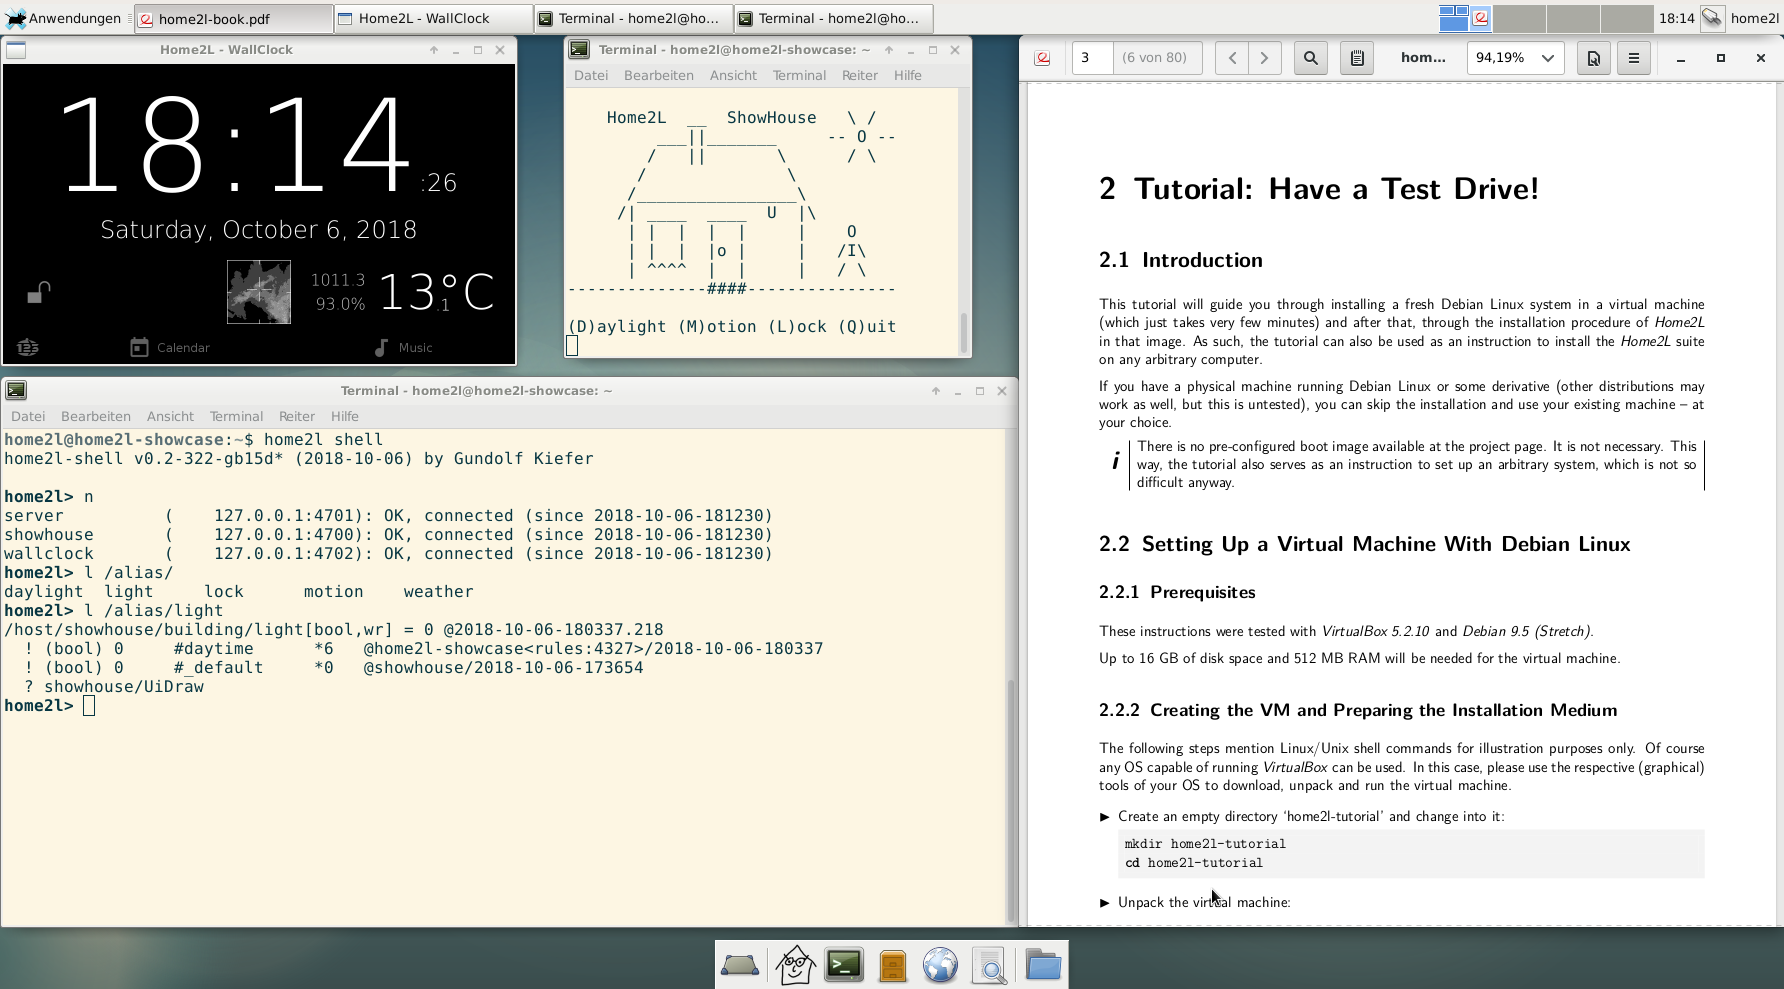
\includegraphics[width=0.95\linewidth,keepaspectratio]{figs/screen-tutorial_layout}
  \caption[l]{Recommended Screen Layout for the Tutorial}
  \label{fig:screen-layout}
\end{figure}


From now on, the terminal window on the upper right is referred to as
the \emph{\textbf{ShowHouse window}}. The lower terminal is referred to as the
\emph{\textbf{Shell window}}.

The \emph{Home2L} suite follows a highly distributed design paradigm. At
this point, there are 4 tools (\emph{Home2L instances}) running
on your machine -- the \emph{ShowHouse}, the \emph{WallClock}, and two background
processes. Together, they simulate a typical, yet simple smart home setup.
The following subsections explain the four instances and their functionalities.

\infobox{
  \textbf{For experienced users:}

  To keep this tutorial simple, all 4 instances are running on the same (virtual) machine.
  Of course, they can arbitrarily be installed on multiple machines. To this end, the
  following configuration settings have be adapted:
  \begin{enumerate}
    \item
      In file \texttt{/opt/home2l/etc/home2l.conf}, section ''Server(s)'':
      Define the local network (\envref{rc.network}) and allow servers to communicate over physical
      interfaces (\envref{rc.serveInterface}).
    \item
      In file \texttt{/opt/home2l/etc/resources.conf}: Edit the section ''Hosts'' accordingly.
    \item
      In file \texttt{/opt/home2l/etc/home2l.conf}, section ''Daemon'': Setup daemon(s) to run the
      appropriate background processes on the respective machine(s).
  \end{enumerate}
}



%%%%%%%%%%%%%%%%%%%%%%%%%%%%%%%%%%%%%%%%%%%%%%%%%%%%%%%%%%%%
\subsection{The \emph{ShowHouse} (\texttt{home2l-showhouse})}
\label{sec:tutorial-firststeps-showhouse}
\toollabel{home2l-showhouse}
%%%%%%%%%%%%%%%%%%%%%%%%%%%%%%%%%%%%%%%%%%%%%%%%%%%%%%%%%%%%

The \emph{ShowHouse} script is a simulator for all physical components
of your tutorial installation: The house and the sun.
The virtual house has the following gadgets:

\begin{enumerate}
\item
  A motion sensor excited if somebody approaches the house.
\item
  A lockable main door with a sensor indicating whether the door is locked or not.
\item
  A door light, which can be switched on or off.
\end{enumerate}

In reality, these would be physical gadgets accessed by respective
\emph{Home2L} hardware drivers -- for example, the GPIO driver (\toolref{home2l-drv-gpio}).
The \emph{ShowHouse} is a Python script containing a \emph{Resource}
driver providing exactly the same interface internally, but lets the
user simulate physical actions by key presses and visualizes the gadgets
with a little ASCII art picture.

In addition to the physical gadgets, the \emph{ShowHouse} script provides
a resource to indicate day/night time. In a real world, this information can
be obtained from the timer driver (see Section~\ref{sec:drvlib-timer})
based on the real time.

\begin{itemize}[$\blacktriangleright$]

\item
  Press the keys listed in the \emph{ShowHouse} window and see how the various gadgets
  (daylight, door lock status, motion) are visualized in the ASCII art.

\end{itemize}

The outdoor light is presently controlled by a background rules script
(see Section~\ref{sec:tutorial-firststeps-rules}).
It is automatically turned on for some time if motion is detected, but only at night time.

\begin{itemize}[$\blacktriangleright$]

\item
  Switch between daylight and night time (press 'D') and simulate motion
  (press 'M') to verify this behavior.

\end{itemize}


\infobox{
  Feel free to inspect the source code of the \emph{ShowHouse}
  (\texttt{/opt/home2l/bin/home2l-showhouse}). It is a Python script and may contain
  a number of useful code examples for writing own rules, drivers or applications.
}



%%%%%%%%%%%%%%%%%%%%%%%%%%%%%%%%%%%%%%%%%%%%%%%%%%%%%%%%%%%%
\subsection{The \emph{WallClock} (\texttt{home2l-wallclock})}
\label{sec:tutorial-firststeps-wallclock}
%%%%%%%%%%%%%%%%%%%%%%%%%%%%%%%%%%%%%%%%%%%%%%%%%%%%%%%%%%%%


The \emph{WallClock} (\toolref{home2l-wallclock}) is the main end user interface --
a universal information display to be mounted on the wall of rooms or installed on mobile devices.

The \emph{WallClock} shows the current time and date in its upper area.
The bottom row contains launcher buttons to access the integrated
calendar and music applets (to be explored later).

Most relevant for this part of the tutorial is the lower part of the
display between the date and the launcher buttons, in which the values of
several sensors -- \emph{Home2L resources} -- are visualized.
These are -- from left to right (referring to Figure~\ref{fig:screen-layout}):

\begin{enumerate}
\item
  Status of the door lock.
\item
  A motion indicator.
\item
  The \emph{radar eye} -- a visualization of weather radar around the building
  (the location is pre-configured for Augsburg, Germany).
\item
  Air pressure and humidity.
\item
  Local outside temperature.
\end{enumerate}

Each of these fields visualizes some \emph{Home2L resource} as
selected in the ''WallClock'' section of \texttt{/opt/home2l/etc/home2l.conf}.
The resources are provided from different sources.

%The \emph{Resources} library can transparently deal with the
%absence of resource data. For example, if the weather driver is absent
%or cannot establish an internet connection to the weather data server,
%the weather-related displays will simply disappear.

\infobox{
  \textbf{Troubleshooting}

  The weather driver depends on an available internet connection and on the \textit{OpenData} server of
  the German Weather Service (DWD). If the server is not reachable at the time you run the
  tutorial, the weather-related displays mentioned above will be missing. If so: Do not worry, the other
  parts of the tutorial are not affected.

  You can diagnose the availabilty of weather data by running the \emph{Weather} driver directly
  in a terminal:
  \lstbox{
    \$ . /opt/env.sh\\
    \$ /opt/home2l/lib/home2l-drv-weather weather.debug=1
  }
}

\begin{itemize}[$\blacktriangleright$]
\item
  In the \emph{ShowHouse} window, push 'M' and observe the motion display in the
  \emph{WallClock} window.
\item
  In the \emph{ShowHouse} window, push 'L' multiple times and see that the
  door lock display in \emph{WallClock} window instantaneously indicates
  the current lock status.
\item
  In the \emph{ShowHouse} window, unlock the door (push 'L' as
  necessary). Then toggle the daylight status (push 'D'). In the
  \emph{WallClock} window, the lock icon is highlighted if the door is
  unlocked at night time to remind the user to keep it locked over night.
\item
  Quit the \emph{ShowHouse} (push 'Q') and see the lock icon
  disappearing in the \emph{WallClock} display. Start the
  \emph{ShowHouse} again (push cursor up and return) and see the lock
  icon re-appearing.

  Repeat this to see that the \emph{WallClock} recognizes
  the presence/absence of resources and servers instantaneously!
\end{itemize}



%%%%%%%%%%%%%%%%%%%%%%%%%%%%%%%%%%%%%%%%%%%%%%%%%%%%%%%%%%%%
\subsection{The Server (\texttt{home2l-server})}
\label{sec:tutorial-firststeps-server}
%%%%%%%%%%%%%%%%%%%%%%%%%%%%%%%%%%%%%%%%%%%%%%%%%%%%%%%%%%%%


This is an instance of the background server (\toolref{home2l-server}),
which in this tutorial hosts the weather driver (\toolref{home2l-drv-weather}).

\infobox{
  In general, \emph{Home2L} does not necessarily need a central server.
  In this example, the weather driver may as well be loaded and executed by \emph{any}
  of the other three \emph{Home2L} instances.

  In practice, however, it may be helpful to distribute the drivers over multiple
  \emph{Home2L} server instances to improve failure resilience, to connect sensors/actors
  to different machines, or for maintenance reasons.

  The assignment of the \emph{weather} driver to the \emph{server} instance is
  configured in the \toolref{home2l.conf} configuration file and may be changed there.
}



%%%%%%%%%%%%%%%%%%%%%%%%%%%%%%%%%%%%%%%%%%%%%%%%%%%%%%%%%%%%
\subsection{The Rules Script (\texttt{rules-showhouse})}
\label{sec:tutorial-firststeps-rules}
%%%%%%%%%%%%%%%%%%%%%%%%%%%%%%%%%%%%%%%%%%%%%%%%%%%%%%%%%%%%


There is presently one automation script active with a rule to
automate the outdoor light.
This script will be explored later in Section \ref{sec:tutorial-rules}.

\begin{itemize}[$\blacktriangleright$]

\item
  Shut down the \emph{Home2L} background services:
  \begin{lstlisting}
    $ sudo systemctl stop home2l
  \end{lstlisting}
  and see that

  \begin{enumerate}[a)]
  \item
    the weather information disappears from the \emph{WallClock} display,
  \item
    the outdoor light no longer switches on automatically on motion at night.
  \end{enumerate}

\item
  Restart the background services
  \begin{lstlisting}
    $ sudo systemctl start home2l
  \end{lstlisting}
  and verify that the weather display and the outdoor light are working properly again.

\end{itemize}


\textbf{Congratuilations!} You have now moved in succesfully into your new house and
tested its basic functionality. Next, we will take a look behind the scenes.





%%%%%%%%%%%%%%%%%%%%%%%%%%%%%%%%%%%%%%%%%%%%%%%%%%%%%%%%%%%%%%%%%%%%%%%%%%
\section{Using the \emph{Home2L Shell}}
\label{sec:tutorial-shell}
%%%%%%%%%%%%%%%%%%%%%%%%%%%%%%%%%%%%%%%%%%%%%%%%%%%%%%%%%%%%%%%%%%%%%%%%%%


This section gives an introduction to the \emph{Home2L Shell} (\toolref{home2l-shell}),
the main command line interface, which we will now use to take a look behind the
scenes. Im particular, we will use the shell to check the status of all
\emph{Home2L} instances, explore the directory tree, manipulate and monitor
resources, and use the shell for logging purposes.

\begin{itemize}[$\blacktriangleright$]
\item
  Go to the \emph{Shell window} and start the \emph{Home2L Shell}:
  \begin{lstlisting}
    $ home2l shell
  \end{lstlisting}
  The shell has an integrated help functionality. Type
  \begin{lstlisting}
    home2l> h
  \end{lstlisting}
  to get a list of available commands or
  \begin{lstlisting}
    home2l> h <command>
  \end{lstlisting}
  to get more detailed information about a certain command.

\item
  Check the status of all servers in the \emph{Home2L} network:
  \begin{lstlisting}
    home2l> n
    server          (    127.0.0.1:4701): OK, connected (since 2018-10-28-194909)
    showhouse       (    127.0.0.1:4700): OK, connected (since 2018-10-28-194909)
    wallclock       (    127.0.0.1:4702): OK, connected (since 2018-10-28-194909)
  \end{lstlisting}
  The list indicates that all servers are OK and reachable from the
  \emph{Home2L Shell}.
\end{itemize}



%%%%%%%%%%%%%%%%%%%%%%%%%%%%%%%%%%%%%%%%%%%%%%%%%%%%%%%%%%%%
\subsection{Navigating and Inspecting Resources}
\label{sec:tutorial-shell-inspect}
%%%%%%%%%%%%%%%%%%%%%%%%%%%%%%%%%%%%%%%%%%%%%%%%%%%%%%%%%%%%


\begin{itemize}[$\blacktriangleright$]
\item
  Use the commands 'c' and 'l' to explore the available resources and the namespace.
  Tab-completion is available.
  List the root directory of the namespace:
  \begin{lstlisting}
    home2l> l /
    alias
    env
    host
    local
  \end{lstlisting}

  The directory \texttt{/host} contains an entry for each host:
  \begin{lstlisting}
    home2l> l /host/
    home2l-showcase<shell:2254>
    server
    showhouse
    wallclock
  \end{lstlisting}

  The directory \texttt{/alias} contains all defined alias names, which are symbolic
  links to host resources or directories:
  \begin{lstlisting}
    home2l> l /alias/
    daylight -> /host/showhouse/building/simDaylight
    light -> /host/showhouse/building/light
    lock -> /host/showhouse/building/lock
    motion -> /host/showhouse/building/motion
    weather -> /host/server/weather
  \end{lstlisting}

  The top-level directory \texttt{/local} is a hard-wired alias to
  \texttt{/host/<self>}, where \texttt{<self>} is the local
  \emph{Home2L} host ID.

\item
  With the 'c' command, you can navigate in the tree.
  \begin{lstlisting}
    home2l> c /alias/light
    /alias/light
  \end{lstlisting}

  \infobox{
    If you are familiar with navigating and exploring files using 'cd', 'ls' and
    tab-completion in a Unix shell: Navigating with the \emph{Home2L Shell} is very
    similar, just easier!
    \begin{enumerate}[a)]
      \item The respective commands have one character instead of two ('c'/'l' instead of 'cd'/'ls').
      \item Tab-completion may auto-complete over multiple directory levels.
      \item The 'l' command does not only list directories, but displays anything (particularly resources, as the next example shows). Simililarly, with 'c' you can not only
        navigate to a directory, but also to a resource itself.
    \end{enumerate}
  }

\item
  The 'l' command without arguments lists the current directory or
  object. Running it now (current location is \texttt{/alias/light})
  displays the outdoor light resource.
  \begin{lstlisting}
    home2l> l
    /host/showhouse/building/light[bool,wr] = 0 @2018-10-28-193047.599
      ! (bool) 1     #motion       *5 -2018-10-28-195452.133   @home2l-showcase<rules:498>/2018-10-28-195447
      ! (bool) 0     #daytime      *6   @home2l-showcase<rules:498>/2018-10-28-193047
      ! (bool) 0     #_default     *0   @showhouse/2018-10-28-193045
      ? showhouse/UiDraw
  \end{lstlisting}

  The first line of the output shows the URI (unified resource indicator)
  of the resource, its type, writability, current value and the time of
  the last change. The next lines list the active requests and
  subscribers.

  Lines starting with an ''!'' show an active request. In the example
  above, there is a request with the ID '\#\_default' for a value of 0
  with a low priority ('*0') and another one '\#motion' for a value of 1
  with a higher priority, which superseeds the default request in this
  situation. The '\#motion' request has a time-out attribute set causing
  the request to be auto-removed at the given time. The '@' tags at the
  end of the lines identify the origin (host/time) for each request.

  \infobox{
    This example reflects the situation shortly after pushing the ''M''
    button in the \textit{ShowHouse} window  at (simulated) daytime.
    The '\#motion' request tries to switch on the light for 5 seconds
    (until 19:54:52). However, a '\#daylight' request at a higher
    priority is active as well, which ties the value to 0, so that the
    light effectively remains off.
  }

  Lines starting with a ''?'' show a subscriber. In this example, there is
  one subscriber, namely the \texttt{'UiDraw()'} function of the \emph{ShowHouse}
  script, which is responsible for redrawing the ASCII art on value
  changes.

\item
  Push ''D'' and ''M'' in the \emph{ShowHouse} to change the daylight
  status and simulate motion (or not) and repeat the above command in
  various situations to see how the respective requests change.

\item
  Explore the directory tree of the installation! Find out, which resources
  available from which of the three \emph{Home2L} server instances!

\end{itemize}



%%%%%%%%%%%%%%%%%%%%%%%%%%%%%%%%%%%%%%%%%%%%%%%%%%%%%%%%%%%%
\subsection{Manipulating Resources Manually}
\label{sec:tutorial-shell-manipulate}
%%%%%%%%%%%%%%%%%%%%%%%%%%%%%%%%%%%%%%%%%%%%%%%%%%%%%%%%%%%%


We now manipulate the light by placing requests manually.

\begin{itemize}[$\blacktriangleright$]

\item
  Enter (\emph{Note: the second command is the digit ''one'', not a
  lower-case ''L''})
  \begin{lstlisting}
    home2l> c /alias/light
    home2l> 1
    /host/showhouse/building/light[bool,wr] = 1 @2018-10-28-201230.940
      ! (bool) 1     #shell        *8   @home2l-showcase<shell:2254>/2018-10-28-201230
      ! (bool) 0     #daytime      *6   @home2l-showcase<rules:498>/2018-10-28-193047
      ! (bool) 0     #_default     *0   @showhouse/2018-10-28-193045
      ? showhouse/UiDraw
  \end{lstlisting}
  and see that the light is turned on. Look at the output: Can you
  identify the request you created with the ''1'' command?

\item
  Make sure that night mode is set in the \emph{ShowHouse} window (push ''D'' as necessary). The
  light will remain on. Then enter
  \begin{lstlisting}
    home2l> 0
    /host/showhouse/building/light[bool,wr] = 0 @2018-10-28-202750.949
      ! (bool) 0     #shell        *8   @home2l-showcase<shell:2254>/2018-10-28-202750
      ! (bool) 0     #_default     *0   @showhouse/2018-10-28-193045
      ? showhouse/UiDraw
  \end{lstlisting}
  This forces the light to stay off. Motion events have no effect on the
  light even at night, since their requests have a lower priority
  (''*6'') than the default priority of shell requests (''*8'').

\item
  Finally, remove the manual shell request by typing
  \begin{lstlisting}
    home2l> -
    /host/showhouse/building/light[bool,wr] = 0 @2018-10-28-202906.524
      ! (bool) 0     #_default     *0   @showhouse/2018-10-28-193045
      ? showhouse/UiDraw
  \end{lstlisting}

\end{itemize}

\infobox{
  The commands ''0'', ''1'', and ''-'' are abbreviations for variants of the ''r+'' and ''r-''
  commands to place and remove requests. More information on this is given in the online help.
}

\begin{itemize}[$\blacktriangleright$]

\item
  It is possible to pass arbitrary request attributes (see Section~\ref{sec:resources-requests})
  as command line arguments. To turn on the light in 2 seconds and off
  again 3 seconds later enter:
  \begin{lstlisting}
    home2l> 1 +2000 -5000
    /host/showhouse/building/light[bool,wr] = 0 @2018-10-28-202906.524
      ! (bool) 1     #shell        *8 +2018-10-28-203449.268 -2018-10-28-203452.268   @home2l-showcase<shell:2254>/2018-10-28-203447
      ! (bool) 0     #_default     *0   @showhouse/2018-10-28-193045
      ? showhouse/UiDraw
  \end{lstlisting}
  The arguments '+2000' and '-5000' add start and stop time attributes to
  the request so that it becomes effective in 2000ms from now until 5000ms
  from now.

\item
  (Optional) Explore the directory tree and watch out for writable resources!

  Can you find out how to dim or switch off the \emph{WallClock} display? \\
  (Hints on this are given below in Section~\ref{sec:tutorial-rules}.)

  Try manipulating the resources, but afterwards, remove all requests again you
  have set in this exercise (''r-'' command).

\end{itemize}



%%%%%%%%%%%%%%%%%%%%%%%%%%%%%%%%%%%%%%%%%%%%%%%%%%%%%%%%%%%%
\subsection{Monitoring Resources}
\label{sec:tutorial-shell-monitor}
%%%%%%%%%%%%%%%%%%%%%%%%%%%%%%%%%%%%%%%%%%%%%%%%%%%%%%%%%%%%


The shell allows to subscribe to any resources using the ''s+'' and ''s-'' commands, respectively.

\begin{itemize}[$\blacktriangleright$]
\item
  Subscribe to all resources provided by the \emph{ShowHouse} building:
  \begin{lstlisting}
    home2l> s+ /host/showhouse/building/*
    Subscriber 'home2l-showcase<shell:7336>/shell'
      /host/showhouse/building/*?
      /host/showhouse/building/light
      /host/showhouse/building/lock
      /host/showhouse/building/motion
      /host/showhouse/building/simDaylight
    : /host/showhouse/building/light = ?
    : /host/showhouse/building/lock = ?
    : /host/showhouse/building/motion = ?
    : /host/showhouse/building/simDaylight = ?
  \end{lstlisting}
  The first part of the output (without the lines starting with '':'')
  shows the ID of the subscriber of the shell and lists the resources it
  currently subscribes to. Lines ending with ''?'' are \emph{watch set}
  entries and are currently not associated with an existing resource.

  \infobox{
    \emph{Watch set} entries may either be named resources or -- as in this case -- wildcard
    patterns. They allow to start and stop the subscribing and serving hosts independently
    from each other. You can verify this by closing both the \emph{ShowHouse} and the \emph{Home2L Shell},
    and then repeating the above command \emph{before} starting the \emph{ShowHouse}.

    The command ''s'' lists the status of the shell's subscriber. Run it before and after starting
    the \emph{ShowHouse}.
  }

  Lines starting with a colon ('':'') are events reported by the
  subscriber. The \emph{Home2L} suite follows a very precise event model.
  Immediately after the subscription, the locally known values are
  reported (''unknown'' in this case). However, in the background,
  the server(s) are contacted. By the time you have read this text,
  the actual values have been delivered from the server(s) to the shell.

\item
  Press return:
  \begin{lstlisting}
    home2l>
    : /host/showhouse/building/light = 0 @2018-11-01-184558.651
    : /host/showhouse/building/light connected
    : /host/showhouse/building/lock = 0 @2018-11-01-184558.651
    : /host/showhouse/building/lock connected
    : /host/showhouse/building/motion = 0 @2018-11-01-184558.651
    : /host/showhouse/building/motion connected
    : /host/showhouse/building/simDaylight = 0 @2018-11-01-184558.651
    : /host/showhouse/building/simDaylight connected
  \end{lstlisting}
  Incoming events are collected in the background and displayed after each shell command.

\item
  To follow and display events immediately when received, run the ''follow'' command:
  \begin{lstlisting}
    home2l> f
  \end{lstlisting}

\item
  Now make some interactions in the \emph{ShowHouse} window
  (e.g.~lock/unlock the door, switch to daytime and move the person).
  The output will be similar to this:
  \begin{lstlisting}
    : /host/showhouse/building/simDaylight = 1 @2018-11-01-184833.883
    : /host/showhouse/building/lock = 1 @2018-11-01-184841.820
    : /host/showhouse/building/lock = 0 @2018-11-01-184846.884
    : /host/showhouse/building/simDaylight = 0 @2018-11-01-184848.494
    : /host/showhouse/building/motion = 1 @2018-11-01-184849.757
    : /host/showhouse/building/light = 1 @2018-11-01-184849.759
    : /host/showhouse/building/motion = 0 @2018-11-01-184850.257
    : /host/showhouse/building/light = 0 @2018-11-01-184854.761
  \end{lstlisting}

\item
  Press \emph{Ctrl-C} to stop ''follow" mode. Events for subscribed resources
  are still reported with their correct time stamps, but only after
  commands have been entered.

\item
  Quit the shell by pressing \emph{Ctrl-D}.

\end{itemize}



%%%%%%%%%%%%%%%%%%%%%%%%%%%%%%%%%%%%%%%%%%%%%%%%%%%%%%%%%%%%
\subsection{Non-Interactive Use and Resource Event Logging}
\label{sec:tutorial-shell-scripting}
%%%%%%%%%%%%%%%%%%%%%%%%%%%%%%%%%%%%%%%%%%%%%%%%%%%%%%%%%%%%


The \emph{Home2L Shell} can also be run in a non-interactive way, so
that certain actions can be performed programmatically from shell
scripts.

\begin{itemize}[$\blacktriangleright$]
\item
  For example, this command turns on the \emph{ShowHouse} light for 2 seconds:
  \begin{lstlisting}
    $ home2l shell -e "c /alias/light; 1 -2000"
  \end{lstlisting}

\item
  To log all motion events, you may use a command like:
  \begin{lstlisting}
    $ home2l shell -e "s+ /alias/motion; f" > motion.log & PID=$!
  \end{lstlisting}
  To stop logging, enter:
  \begin{lstlisting}
    $ kill $PID
  \end{lstlisting}

\item
  To log the outside temparature over time, run:
  \begin{lstlisting}
    $ home2l shell -e "s+ /alias/weather/temp; f"
  \end{lstlisting}
  (Again, this job may optionally be backgrounded and its output
  redirected as in the previous example.)

\end{itemize}





%%%%%%%%%%%%%%%%%%%%%%%%%%%%%%%%%%%%%%%%%%%%%%%%%%%%%%%%%%%%%%%%%%%%%%%%%%
\section{\emph{WallClock} Gadgets: The Music Player}
\label{sec:tutorial-wallclock}
%%%%%%%%%%%%%%%%%%%%%%%%%%%%%%%%%%%%%%%%%%%%%%%%%%%%%%%%%%%%%%%%%%%%%%%%%%


The \emph{WallClock}'s music player is a
\href{https://www.musicpd.org/}{Music Player Daemon (MPD)} client,
optimized for a home setup with multiple \emph{WallClocks} in different
rooms and multiple music machines. For this tutorial, the server has been already
installed and started during the previous steps.

\begin{itemize}[$\blacktriangleright$]
\item
  Copy some of favorite \emph{mp3} files into
  \begin{lstlisting}
    /var/opt/home2l/mpd/music
  \end{lstlisting}
  Alternatively, you can download some free music from \url{https://freemusicarchive.org},
  for example.

\item
  Update the \emph{MPD} database
  \begin{lstlisting}
    $ mpc -h localhost update
  \end{lstlisting}

\item
  Increase the size of the \emph{WallClock} (\emph{F10} or \emph{F11})
  and push the \emph{''Music''} button.

\item
  With the player selection button on the bottom, select
  \emph{''ShowStage''}.

\item
  In the navigation pane (right half of the screen), navigate to your
  favorite song. Pushing the title bar of the navigation pane will
  navigate up or switch between the local database and playlists.

\item
  Select your favorite song, push the play button and enjoy!

\end{itemize}


\infobox{
  \textbf{Troubleshooting}

  The integrated music player relies on a working MPD (should have been installed so far)
  and a working audio output of your virtual machine (VM).

  The MPD configuration file is located in \texttt{/opt/home2l/etc/mpd-showstage.conf}. It
  should work out-of-the-box, but may (have to) be further adapted to your preferences.
  By default, the audio output is directed to the default ALSA playback channel.

  To test if audio playback is working inside your VM, run:
  \lstbox{
    \$ speaker-test -t sine
  }

  To adjust the volume, run:
  \lstbox{
    \$ alsamixer
  }

  To update the music database after you have copied files into the music directory:
  \lstbox{
    \$ mpc -h localhost update
  }

  Make sure that the \emph{MPD} instance with the \emph{Home2L} configuration has been started properly
  and that the default instance is off:
  \lstbox{
    \$ sudo systemctl disable mpd \\
    \$ sudo systemctl stop mpd \\
    \$ sudo systemctl restart home2l
  }
}





%%%%%%%%%%%%%%%%%%%%%%%%%%%%%%%%%%%%%%%%%%%%%%%%%%%%%%%%%%%%%%%%%%%%%%%%%%
\section{\emph{WallClock} Gadgets: The Family Calendar}
\label{sec:tutorial-calendar}
%%%%%%%%%%%%%%%%%%%%%%%%%%%%%%%%%%%%%%%%%%%%%%%%%%%%%%%%%%%%%%%%%%%%%%%%%%


The calender applet uses \texttt{remind(1)} as a backend and thus
supports its syntax for specifying events.

\begin{itemize}[$\blacktriangleright$]
\item
  Increase the size of the \emph{WallClock} (\emph{F10} or \emph{F11})
  and start the applet by pushing ''Calendar'' on the main screen.
\item
  Explore the calendar UI by navigating to different dates (e.g.~your wife's
  next birthday or your next anniversary).
\item
  Select an event in the right pane and modify it (e.g.~change its time
  or text).
\item
  Select a day in the left pane and add a new one-time appointment for
  Julian, for example (enter/keep your own date at the beginning):
  \begin{lstlisting}
    2018-12-23 at 19:00 dur 2:00 MSG Meet Henry; Murphy's Pub
  \end{lstlisting}
\end{itemize}





%%%%%%%%%%%%%%%%%%%%%%%%%%%%%%%%%%%%%%%%%%%%%%%%%%%%%%%%%%%%%%%%%%%%%%%%%%
\section{Writing Automation Rules}
\label{sec:tutorial-rules}
%%%%%%%%%%%%%%%%%%%%%%%%%%%%%%%%%%%%%%%%%%%%%%%%%%%%%%%%%%%%%%%%%%%%%%%%%%


This section introduces the development of automation rules. \emph{Home2L rules}
are normal Python scripts. They can be tested separately from already
existing rules files and later be merged into them.

\begin{itemize}[$\blacktriangleright$]

\item
  Make sure that the \emph{WallClock} window is small (push \emph{F9})
  and the screen layout is as sketched in Figure~\ref{fig:screen-layout}.
  The \emph{ShowHouse} must be running, and in the
  \emph{Shell window}, a normal command prompt must be active (quit the
  \emph{Home2L Shell}, if it is still running).

\item
  Inspect and read the supplied rules file:
  \begin{lstlisting}
    $ sudo nano /opt/home2l/etc/rules-showhouse
  \end{lstlisting}

  Can you identify the rules for controlling the light?

  What would you need to change to increase the light-on duration after a motion event?
  How is the light kept off at day time?

\item
  Identify the rule for keeping the \emph{WallClock} permanently active
  \begin{lstlisting}
    @daily("wallclock")
    def PermanentRules (host):
      ...
  \end{lstlisting}
  and deactivated it by commenting out the first line with the
  \texttt{@daily} decorator:
  \begin{lstlisting}
    # @daily("wallclock")
    def PermanentRules (host):
      ...
  \end{lstlisting}
  Exit \texttt{nano} and save the file (\emph{Ctrl-X}).

\item
  To make this change effective, restart the modified rules script
  \texttt{rules-showhouse} and remove its permanent request:
  \begin{lstlisting}
    $ pkill rules-showhouse
    $ home2l shell -e "c /host/wallclock/ui; r- active rules; r- standby rules"
  \end{lstlisting}

\end{itemize}

After some time (at most 10 seconds, see the \envref{ui.standbyDelay} setting in
\toolref{home2l.conf}), the \emph{WallClock} UI should dim or turn off
completely. Clicking on it re-activates it for some time. You may test
this now, but should then wait again until the screen dims. After that,
you should not click into the \emph{WallClock} window anymore.

\infobox{
  Like potentially any \emph{Home2L} application, the \emph{WallClock}
  exports a number of resources. For example, on \emph{Android} it can export
  the device's brightness sensor value or Bluetooth status. In this tutorial, we will use
  \rcref{ui/active}, \rcref{ui/standby} for controlling the UI state and optionally
  \rcref{ui/mute} to mute the audio player.
}

\begin{itemize}[$\blacktriangleright$]

\item
  Setup all necessary environment variables and start an interactive Python session:
  \begin{lstlisting}
    $ . /opt/home2l/env.sh
    $ python3
  \end{lstlisting}

  \end{itemize}

Inside this session, we will now develop a new rule to control the
active/standby state the \emph{WallClock} application.

\infobox{
  Instead of working in the interactive shell, you can, of course, enter the
  Python commands of the following instructions into the \texttt{rules-showhouse}
  file or into a new file. A new file can be generated as follows:
  \lstbox{
    \$ echo '\#!/usr/bin/python3' > myrules \\
    \$ chmod a+x myrules
  }
  This is particularly useful if you intend to experiment with the rules and change them.
}

Enter all following instructions at the Python command prompt
(\lst{\mbox{\textgreater}\mbox{\textgreater}\mbox{\textgreater}}).
The prompt is not always printed in the following instructions to facilitate copy-and-paste.

\begin{itemize}[$\blacktriangleright$]

\item
  Import the \emph{Home2L} package and initialize it:
  \begin{lstlisting}
    from home2l import *
    Home2lInit ("myrules")
  \end{lstlisting}

\item
  Get references to all resources used later:
  \begin{lstlisting}
    rcDaylight = RcGet ("/alias/daylight")
    rcLock = RcGet ("/alias/lock")
    rcUiActive = RcGet ("/host/wallclock/ui/active")
  \end{lstlisting}

\item
  (Optional) In an interactive Python shell, you can now inspect the network
  environment and resources:
  \begin{lstlisting}[language=Python]
    >>> Home2lStart ()    # Start the Home2L background tasks
    >>> RcHosts ()
    ['home2l-showcase<python:6862>', 'server', 'showhouse', 'wallclock']
    >>> RcHostResources ("wallclock")
    ['/host/wallclock/timer/daily', '/host/wallclock/timer/hourly', '/host/wallclock/timer/minutely', '/host/wallclock/timer/now', '/host/wallclock/timer/twilight/dawn06', '/host/wallclock/timer/twilight/dawn12', '/host/wallclock/timer/twilight/dawn18', '/host/wallclock/timer/twilight/day', '/host/wallclock/timer/twilight/day06', '/host/wallclock/timer/twilight/day12', '/host/wallclock/timer/twilight/day18', '/host/wallclock/timer/twilight/dusk06', '/host/wallclock/timer/twilight/dusk12', '/host/wallclock/timer/twilight/dusk18', '/host/wallclock/timer/twilight/sunrise', '/host/wallclock/timer/twilight/sunset', '/host/wallclock/ui/active', '/host/wallclock/ui/bluetooth', '/host/wallclock/ui/bluetoothAudio', '/host/wallclock/ui/dispLight', '/host/wallclock/ui/luxSensor', '/host/wallclock/ui/mute', '/host/wallclock/ui/standby']
    >>> rcDaylight
    (CResource) /host/showhouse/building/simDaylight bool ro
  \end{lstlisting}
  Of course, online help and tab-completion is available for all commands. For example, try:
  \begin{lstlisting}
    >>> help (RcGet)
    Help on function RcGet in module home2l:

    RcGet(uri, allowWait=False)
        RcGet(char const * uri, bool allowWait=False) -> CResource
        RcGet(char const * uri) -> CResource

        Lookup a resource by its URI and return a reference to it.
  \end{lstlisting}

\item
  Define a rule which switches on the display whenever the door is unlocked at night
  (mind the indentation!):
  \begin{lstlisting}
  >>> @onUpdate(rcDaylight, rcLock)
  ... def UpdateUiState ():
  ...   print ("### daylight = " + str (rcDaylight.ValueState ())
  ...              + ", lock = " + str (rcLock.ValueState ()))
  ...   daylight = rcDaylight.ValidValue (False)
  ...   doorLocked = rcLock.ValidValue (False)
  ...   if not daylight and not doorLocked:
  ...     rcUiActive.SetRequest (value = True)
  ...   else:
  ...     rcUiActive.DelRequest ()
  ...
  \end{lstlisting}

  The first line (''\texttt{@update()}''), a Python \emph{decorator},
  makes the function \texttt{UpdateUiActive()} to be called whenever
  the value of any of the supplied resources changes. Inside the function
  body, the values of \texttt{rcDaylight} and \texttt{rcLock} are
  read using the \texttt{ValidValue()} method, which takes a default
  value as an argument and always returns a valid value, even if the
  actual resource value is currently unknown. Depending on these values, a
  request is set to switch the display active or not.

\item
  (Optional) Define another rule to mute the music player for 5 seconds
  if motion is detected in front of the house:
  \begin{lstlisting}
    >>> @onEvent ("/alias/motion")
    ... def MuteOnMotion (ev, rc, vs):
    ...   if ev == rceValueStateChanged and vs.ValidValue (False) == True:
    ...     RcSetRequestFromStr ("/host/wallclock/ui/mute", "1 -5000")
    ...
  \end{lstlisting}

  For demonstration purposes, this example uses some other API functions
  than the previous ones:
  \begin{itemize}
    \item
      Instead of \texttt{@onUpdate()}, the \texttt{@onEvent()} decorator is used,
      which allows to precisely track all events.
    \item
      The resources are directly identified by their URI without first getting
      an object reference by \texttt{RcGet()}.
    \item
      The request is set by \texttt{RcSetRequestFromStr()}, which allows to describe the request
      by a string with the same syntax as already known from the \emph{Home2L Shell}.
  \end{itemize}
  Details can be found in the \refapipython{} and in Section~\ref{sec:resources-syntax}.

\item
  Run the \emph{Home2L} main loop:
  \begin{lstlisting}
  Home2lRun()
  \end{lstlisting}
  The new rule(s) are now active.

\item
  Test the new rule(s) by interacting with the \emph{ShowHouse}!

\end{itemize}





%%%%%%%%%%%%%%%%%%%%%%%%%%%%%%%%%%%%%%%%%%%%%%%%%%%%%%%%%%%%%%%%%%%%%%%%%%
\section{Going Further}
\label{sec:tutorial-goingfurther}
%%%%%%%%%%%%%%%%%%%%%%%%%%%%%%%%%%%%%%%%%%%%%%%%%%%%%%%%%%%%%%%%%%%%%%%%%%


To learn more about the capabilities of the \emph{Home2L} suite, we
suggest to look into the configuration files and source code of the
tutorial.

\begin{itemize}[$\blacktriangleright$]

\item
  The supplied rules file has already been inspected in Section~\ref{sec:tutorial-rules}:
  \begin{lstlisting}
    $ nano /opt/home2l/etc/rules-showhouse
  \end{lstlisting}

\item
  Inspect and read the \emph{ShowHouse} source file:
  \begin{lstlisting}
    $ nano /opt/home2l/bin/home2l-showhouse
  \end{lstlisting}

  It contains an example for a resource driver implemented in Python,
  namely for the \emph{ShowHouse} gadgets and the keyboard input. The
  latter is a bit more sophisticated and involves a background thread.

  The ASCII art visualization is refreshed whenever necessary, but not
  unnecessarily often. This is achieved by implementing the drawing function as a rule.

\item
  Inspect or read the main configuration file
  \begin{lstlisting}
    $ nano /opt/home2l/etc/home2l.conf
  \end{lstlisting}

\end{itemize}

Feel free to modify any of these or other files to learn more about
their options. If you change a configuration file, it may be necessary
to restart the \emph{Home2L} background services for the changes to take
effect.

If you are using the \emph{systemd} init system (as in the \emph{Home2L
ShowCase} VM used here), the \emph{Home2L} Daemon with all its services
is restarted by the following command:

\begin{lstlisting}
  $ systemctl restart home2l
\end{lstlisting}

If you are using the \emph{System-V} init system, the \emph{Home2L Daemon}
is restarted by:

\begin{lstlisting}
  $ service home2l restart
\end{lstlisting}

A shortcut to restart just a single instance -- for example, the
\emph{home2l-rules} script -- is to simply kill that instance. It will
be restarted automatically by the \emph{Home2L Daemon}.

\begin{lstlisting}
  $ pkill home2l-rules
\end{lstlisting}





%%%%%%%%%%%%%%%%%%%%%%%%%%%%%%%%%%%%%%%%%%%%%%%%%%%%%%%%%%%%%%%%%%%%%%%%%%%%%%%
%
\chapter{Compiling and Installing}
\label{ch:installing}
%
%%%%%%%%%%%%%%%%%%%%%%%%%%%%%%%%%%%%%%%%%%%%%%%%%%%%%%%%%%%%%%%%%%%%%%%%%%%%%%%




%%%%%%%%%%%%%%%%%%%%%%%%%%%%%%%%%%%%%%%%%%%%%%%%%%%%%%%%%%%%%%%%%%%%%%%%%%
\section{Overview}
\label{sec:installing-intro}
%%%%%%%%%%%%%%%%%%%%%%%%%%%%%%%%%%%%%%%%%%%%%%%%%%%%%%%%%%%%%%%%%%%%%%%%%%


\emph{Home2L} comes with its own build system. This is accounts for
the fact that \emph{Home2L} is not a piece of software to be installed
on a single computer, but instead, the \emph{Home2Ls} are installed in a
''home'', which is a heterpgeneous \emph{cluster} of machines with
different hardware (e.g.~x86, ARM) and operating software environments.

The build system is therefore capable for cross-compilation. Presently,
it assumes a Debian-based environment and is tested under Debian 9.x
(Stretch).





%%%%%%%%%%%%%%%%%%%%%%%%%%%%%%%%%%%%%%%%%%%%%%%%%%%%%%%%%%%%%%%%%%%%%%%%%%
\section{Prerequisites}
\label{sec:installing-prerequisites}
%%%%%%%%%%%%%%%%%%%%%%%%%%%%%%%%%%%%%%%%%%%%%%%%%%%%%%%%%%%%%%%%%%%%%%%%%%


The requirements for building the core part of the \emph{Home2Ls} are
quite small:

\begin{itemize}
\item
  A C/C++ compiler (compliant with the \emph{C99} and \emph{C++11} standards)
  with basic libraries (\texttt{libc}, \texttt{libstdc++}).
\item
  \emph{Python 3} with development packages and \emph{SWIG}
  (\textgreater{}= 3) for the \emph{Python API}.
\item
  \texttt{libreadline} (optional, for the \toolref{home2l-shell}).
\end{itemize}

Section~\ref{sec:tutorial-prerequisites} provides an exact list of
packages to install on Debian or Debian-based systems.

Building the documentation (module '\texttt{doc}') requires a couple
of additional packages (\texttt{doxygen, texlive, graphviz, ...}).
Most users do not have to build the documentation, since readable
versions are available on the project page.



%%%%%%%%%%%%%%%%%%%%%%%%%%%%%%%%%%%%%%%%%%%%%%%%%%%%%%%%%%%%
\subsection{Cross-Compilation}
\label{sec:installing-cross}
%%%%%%%%%%%%%%%%%%%%%%%%%%%%%%%%%%%%%%%%%%%%%%%%%%%%%%%%%%%%


Cross-compilation is supported by the \emph{Home2L} build system based
on the Debian cross-building capabilities for the architectures
\texttt{i386}, \texttt{amd64}, and \texttt{armhf}. The
development machine must have \texttt{i386} or \texttt{amd64} as
its primary architecture. The other architectures must be entered as
additional architectures to the \texttt{dpkg(1)} package manager

To cross-build \texttt{armhf} binaries on an \texttt{i386} or
\texttt{amd64} machine, as of Debian 9 (''Stretch''), the following packages
must be installed:

\begin{lstlisting}
crossbuild-essential-armhf g++-6-multilib
\end{lstlisting}

For all desired target architectures, the respective development packages mentioned above must be installed.
.



%%%%%%%%%%%%%%%%%%%%%%%%%%%%%%%%%%%%%%%%%%%%%%%%%%%%%%%%%%%%
\subsection{Optional External Libraries}
\label{sec:installing-external}
%%%%%%%%%%%%%%%%%%%%%%%%%%%%%%%%%%%%%%%%%%%%%%%%%%%%%%%%%%%%


Some applications require additional external libraries, sometimes
depending on the options they are compiled with, as indicated in
Figure~\ref{fig:home2l-components}. The folder
\texttt{externals/} in the source tree contains hints on how to
obtain, build and setup the respective libraries for different
platforms. Please note, that this folder is distributed ''as is''
without any warranty and may potentially be incomplete. Files to watch for are:

\begin{description}
\item[\texttt{prebuild.sh}:]
  A build script with comments on how to obtain the sources and hints for building.
\item[\texttt{Debian.mk}:]
  A Debian/Linux makefile fragment.
\item[\texttt{Android.mk}:]
  An Android NDK makefile fragment.
\end{description}





%%%%%%%%%%%%%%%%%%%%%%%%%%%%%%%%%%%%%%%%%%%%%%%%%%%%%%%%%%%%%%%%%%%%%%%%%%
\section{Compiling}
\label{sec:installing-compiling}
%%%%%%%%%%%%%%%%%%%%%%%%%%%%%%%%%%%%%%%%%%%%%%%%%%%%%%%%%%%%%%%%%%%%%%%%%%


To build and install the suite, do the following:

\begin{enumerate}
\item
  View the build options by running the following command in the main
  source directory to view the build options:
  \begin{lstlisting}
  $ make help
  \end{lstlisting}
\item
  Check and, if necessary, adapt the compiler and build settings in file \texttt{Setup.mk}.
\item
  Build:
  \begin{lstlisting}
  $ make <options>
  \end{lstlisting}
\item
  Install the \emph{blob} to \texttt{\$HOME2L\_ROOT} (default:
  \texttt{/opt/home2l}):
  \begin{lstlisting}
  $ make <options> install
  \end{lstlisting}
\end{enumerate}

This will install the so-called \emph{Home2L blob} on your computer. It
contains all files for all architectures together with a sample
configuration (in \texttt{\$HOME2L\_ROOT/etc/}). This \emph{blob} can now be simply
copied to all machines of your cluster. The \toolref{home2l-rollout} tool
can automate that for software or configuration updates.
To use the \emph{Home2Ls}, some additional things have to be set up.
This is explained in the following sections.





%%%%%%%%%%%%%%%%%%%%%%%%%%%%%%%%%%%%%%%%%%%%%%%%%%%%%%%%%%%%%%%%%%%%%%%%%%
\section{Setting Up Users and Permissions}
\label{sec:installing-users}
%%%%%%%%%%%%%%%%%%%%%%%%%%%%%%%%%%%%%%%%%%%%%%%%%%%%%%%%%%%%%%%%%%%%%%%%%%



\subsection{Users and Groups}

The following users are involved and must exist on each machine:

\begin{itemize}
\item
  User \texttt{'home2l'} with primary group \texttt{'home2l'}: Under this
  UID, all \emph{Home2L} background processes are executed. This user should get
  all permission required for its background or end-user tasks, but no more than that.
  In particular, \texttt{'home2l'} should not be allowed to modify configuration files.
\item
  User \texttt{'root'}: The super user.
\item
  The user account of the administrating user - we call her \texttt{'myadmin'} here.
\end{itemize}

The user \texttt{'home2l'} must have \texttt{'bash'} as its login shell and the following
line in its \texttt{.bashrc} file to have all \texttt{'HOME2L\_*'} environment variables set
when required:
\begin{lstlisting}
source $(home2l -e)
\end{lstlisting}



\subsection{Automatic \texttt{ssh} Logins \texttt{sudo} Rules for Cluster Administration}

For central cluster adminstration using \toolref{home2l-rollout}, the following
\emph{sudo} rules are required on each machine of the cluster:
\begin{itemize}
  \item
    for \texttt{'myadmin'}: run \toolref{home2l-install} as \texttt{'root'}
  \item
    for \texttt{'myadmin'}: run \texttt{adb(1)} as \texttt{'home2l'} (only on machines hosting Android devices)
  \item
    for \texttt{'home2l'}: run \toolref{home2l-sudo} as \texttt{'root'} (optional)
\end{itemize}

The following \emph{ssh} logins must be possible without a password in the cluster (''\texttt{master}'' is the master machine):
\begin{itemize}
\item
  from \texttt{'myadmin@master'} to any other machine as user \texttt{'myadmin'},
\item
  from \texttt{'root'} at any non-master host to \texttt{'home2l@master'}.
\end{itemize}



\subsection{File Permissions}

The file permissions in the installation directory (including \texttt{etc/}) are maintained
by the tools \toolref{home2l-install} and \toolref{home2l-rollout} as follows:
\begin{itemize}
  \item
    \toolref{home2l-install} sets the ownership to \texttt{'root:home2l'}.
    Permissions are preserved from the master, \texttt{'make install'} sets them to
    644 for files and 755 for directories.
  \item
    The folder \texttt{etc/secrets} is meant for storing sensitive data only readable by
    members of the group \texttt{'home2l'}.
    The permissions are set to 640 for files and 750 for directories.
    Hence, only \texttt{'root'} or users of group \texttt{'home2l'} can read them, and only
    \texttt{'root'} can modify them. Others have no access.
\end{itemize}






%%%%%%%%%%%%%%%%%%%%%%%%%%%%%%%%%%%%%%%%%%%%%%%%%%%%%%%%%%%%%%%%%%%%%%%%%%
\section{Adding a New Machine to the Cluster}
\label{sec:installing-newhost}
%%%%%%%%%%%%%%%%%%%%%%%%%%%%%%%%%%%%%%%%%%%%%%%%%%%%%%%%%%%%%%%%%%%%%%%%%%


To install the \emph{Home2L} suite on the first computer, follow the building
and installation steps described Section~\ref{sec:installing-compiling} to install
a \emph{Home2L blob} on your \emph{master computer}. To complete the installation,
run (assuming that the blob is installed in \texttt{/opt/home2l}):
\begin{lstlisting}
$ sudo /opt/home2l/bin/home2l-install -i
\end{lstlisting}

The tool explains itself what it is doing.

To prepare a new additional (Linux) machine and add it to the cluster, the
installation blob can be cloned from an existing (typically the \emph{master}) machine.

\begin{enumerate}
  \item
    On the \emph{master}: Edit the configuration files \toolref{rollout.conf},
    \toolref{install.conf} and \toolref{init.conf} to reflect the new setup
    with the new machine.
  \item
    On the new machine: Setup users and their rights as described in Section~\ref{sec:installing-users}.
  \item
    On the new machine: Replicate the blob from the master by running a command like
    \begin{lstlisting}
    $ sudo rsync -va --perms --chown=root:home2l home2l@master:/opt/home2l/ /opt/home2l
    \end{lstlisting}
  \item On the new machine, run:
    \begin{lstlisting}
    $ sudo /opt/home2l/bin/home2l-install -i
    \end{lstlisting}
  \item
    On the master, run
    \begin{lstlisting}
    $ home2l-rollout
    \end{lstlisting}
    and check, if the new machine is listed. Press 'y' (''yes'') to run the rollout procedure
    and see if updating the new machine works without errors.
\end{enumerate}

From now on, software and configuration updates can be rolled out by the tool
\toolref{home2l-rollout} from the master.





%%%%%%%%%%%%%%%%%%%%%%%%%%%%%%%%%%%%%%%%%%%%%%%%%%%%%%%%%%%%%%%%%%%%%%%%%%
\section{Installing the \emph{WallClock} on Android}
\label{sec:installing-android}
%%%%%%%%%%%%%%%%%%%%%%%%%%%%%%%%%%%%%%%%%%%%%%%%%%%%%%%%%%%%%%%%%%%%%%%%%%


\warnbox{
  This section is under construction.

  Compiling and installing the \emph{Android} app presently requires good knowledge in
  programming and \emph{Android} debugging. The following text is only a brief sketch on what to do (see Section~\ref{sec:helping}).
}

To set up an \emph{Android} hosts, for example a \emph{WallClock} tablet, the following
steps have to be done:

\begin{enumerate}
  \item \emph{Not strictly necessary, but recommended:} Install a Linux distribution
    environment on the Android device (e.g.~using \emph{Lil'Debi} or \emph{Linux Deploy}).
    Then install \emph{Home2L} into this environment as described in Section~\ref{sec:installing-newhost}.
    Install the blob to \lst{/data/home2l} (not \texttt{/opt/home2l}). This allows to
    use the same blob from the app and the Linux distribution environment.

    This environment allows you to:
    \begin{itemize}
      \item use the \emph{WallClock} calendar applet,
      \item see the system info on the \emph{WallClock} system info screen,
      \item use \toolref{home2l-rollout} to maintain this machine,
      \item use the \emph{Home2L} command line tools in this environment.
    \end{itemize}

  \item \emph{If you do not have a Linux distribution environment (previos step):}
    Copy the \emph{Home2L blob} to \lst{/data/home2l} (e.g. using \texttt{adb(1)}).

  \item Install the \emph{WallClock} Android app.

  \item For some of the functionality mentioned in step 1, the Android app needs to run commands
    in the Linux distribution environment. This is done by SSH logins from the Android
    environment into the Linux distribution environment. To set this up:
    \begin{enumerate}[a)]
      \item Generate an SSH identity without a password and store it as
        \texttt{'etc/secrets/ssh/<hostname>[.pub]'}.
      \item In the Linux distribution environment, install an SSH daemon and allow logins without
        password from \texttt{'localhost'} as user \texttt{'home2l'}.
      \item Test the connection from an Android shell:
        \begin{lstlisting}[language=bash]
        $ adb shell
        $ su   # to make etc/secrets/ssh/* accessible
        # ssh -i /data/home2l/etc/secrets/ssh/mymachine  -o NoHostAuthenticationForLocalhost=yes home2l@localhost
            # Replace 'mymachine' with the hostname of your Android machine.
            # A shell in the Linux distribution environment should open.
        mymachine: $ $HOME2L_ROOT/bin/h2l-sysinfo.sh
            # This should print a list of processes and further system information.
        \end{lstlisting}
    \end{enumerate}
    Similar to what is mentioned in Section~\ref{sec:installing-users}, \toolref{home2l-install}
    maintains the file permissions in \texttt{etc/secrets} in a special way, with the following
    additions on Android:
    \begin{itemize}
      \item
        The ownership is set to the UID of the \emph{Home2L WallClock} Android app.
      \item
        The folder \texttt{'etc/secrets/ssh'} and its contents are set group-inaccessible,
        so that nobody but the \emph{WallClock} app owner (and \texttt{root}) can read the
        SSH IDs.
    \end{itemize}
\end{enumerate}

If the \emph{WallClock} app fails to start due to some configuration problems,
detailed information for diagnosis can be found in the Android log system. This can be
viewed using \texttt{adb(1)}:
\begin{lstlisting}
$ adb logcat -v time home2l:D SDL:V *:E *:W *:I
\end{lstlisting}





%%%%%%%%%%%%%%%%%%%%%%%%%%%%%%%%%%%%%%%%%%%%%%%%%%%%%%%%%%%%%%%%%%%%%%%%%%
\chapter{Managing a \emph{Home2L} Installation}
\label{ch:managing}
%%%%%%%%%%%%%%%%%%%%%%%%%%%%%%%%%%%%%%%%%%%%%%%%%%%%%%%%%%%%%%%%%%%%%%%%%%


A typical \emph{Home2L} installation is distributed over multiple
computers (\emph{machines}), on each of which one ore multiple \emph{Home2l instances}
may be running. There is no central server, all \emph{Home2L instances} are equal in rank.





%%%%%%%%%%%%%%%%%%%%%%%%%%%%%%%%%%%%%%%%%%%%%%%%%%%%%%%%%%%%%%%%%%%%%%%%%%
\section{Terminology}
\label{sec:managing-terminology}
%%%%%%%%%%%%%%%%%%%%%%%%%%%%%%%%%%%%%%%%%%%%%%%%%%%%%%%%%%%%%%%%%%%%%%%%%%


In this document, the following terminology is used:

\begin{description}

\item[A \emph{machine}]
  is a physical computer.

\item[A \emph{Home2L instance}]
  is a running program (process) using the \emph{Home2L} library, such as
  \toolref{home2l-wallclock}, \toolref{home2l-shell},
  or a rules script. Each instance is identified by its \textbf{\emph{instance name}}
  (or \emph{instance ID}),
  which is typically the name of its executable (without a leading ''home2l-''),
  but may be set to a different value by the respective application
  (see \envref{sys.instanceName}). The instance name must be unique on a machine.

\item[A \emph{Home2L cluster}]
  (or \emph{Home2L network}) is a set of machines running \emph{Home2L} instances
  that interact with each other and make up the \emph{Home2L} installation.

\item[The \emph{master}] machine is the computer from which a cluster is managed,
  typically the desktop PC of the adminstrator.
  From this machine, software and configuration updates are rolled out.

\item[A \emph{Home2L server}]
  is an instance exporting \emph{Home2L} resources (see Chapter~\ref{ch:resources}).

\item[A \emph{Home2L client}]
  is an instance accessing resources (i.e. any process incorporating the
  \emph{Home2L Resources} library).

\item[A \emph{Home2L host}]
  a \emph{Home2L} server or client, in other words: an instance communicating in a
  \emph{Home2L cluster}.
  It is identified by the \textbf{\emph{host ID}} as declared in \toolref{resources.conf}.

\end{description}

\infobox{
  The term \emph{'host'} is frequently used as a synonym for a computer or machine.
  However, its meaning may as well differ slightly. For example,
  \begin{enumerate}[a)]
    \item a \emph{host name} may refer to an IP address in a network, and as such identify
      an interface of a computer, not the computer itself, which may have
      multiple interfaces.
    \item the term \emph{host} may refer to the operating system running on physical
      hardware as opposed to the guest operating sytem running in a virtual machine
      on the same hardware.
  \end{enumerate}

  In the \emph{Home2L} context, a \emph{host} actually refers to a \emph{Home2L} instance
  running on a machine.
  Often, there is only one instance running per machine, so that its host ID is equivalent
  to the machine name (aka ''hostname''). However, there may as well be multiple servers with
  different \emph{host IDs}.

  To avoid ambiguities, this book avoids to use the term \emph{host} for anything other than
  a \emph{Home2L host}, even if it is common to call a machine ''host'', speaking
  of a ''hostname'' as the name identifying a machine etc. .
}





%%%%%%%%%%%%%%%%%%%%%%%%%%%%%%%%%%%%%%%%%%%%%%%%%%%%%%%%%%%%%%%%%%%%%%%%%%
\section{Common Maintenance Tools}
\label{sec:managing-tools}
\toollabel{home2l-install}
\toollabel{home2l-rollout}
\toollabel{home2l-sudo}
\toollabel{home2l-adb}
%%%%%%%%%%%%%%%%%%%%%%%%%%%%%%%%%%%%%%%%%%%%%%%%%%%%%%%%%%%%%%%%%%%%%%%%%%


The common tools for maintaining \emph{Home2L} installations are:

\begin{itemize}
\item
  \textbf{\toolref{home2l-shell}:} The command line interface
  and ''swiss army knife'' to access and inspect the \emph{Home2L}
  resources. Details can be found in Section~\ref{sec:shell}.
\item
  \textbf{\toolref{home2l-rollout}:} Tool to distribute configuration
  changes or software updates from the master to the other machines.
\item
  \textbf{\toolref{home2l-install}:} Internal tool for performing
  various installation tasks on the local machine. This tool is usually not
  called manually, but indirectly by \toolref{home2l-rollout}.
\item
  \textbf{\toolref{home2l-sudo}:} (optional) Container to allow the
  \texttt{home2l} user to perform a limited set tasks with
  \texttt{root} privileges (e.g.~to restart certain system services
  if they fail to ensure long-term availability). The use of this tool
  is optional, to use it, the file \texttt{/etc/sudoers} has to be
  set up such that \texttt{home2l} can run it as \texttt{root}.
  The allowed activities are encoded in the tool itself. Please note,
  that the tool is presently implemented as a shell script and therefore
  prone to (yet unknown) potential security holes.
\item
  \textbf{\toolref{home2l-adb}:} (optional) Wrapper for the \emph{Android Debug
  Bridge (ADB)}, allows to maintain Android machines connected by USB cable
  to Linux machines (requires \toolref{androidb.conf} to be set up).
\end{itemize}

Each of the tools implements a \texttt{-h} (help) option, which gives up-to-date usage information.

Tools can be invoked in one of two ways:

\begin{enumerate}[a)]

\item
  Calling the tool directly after setting the \emph{Home2L} environment settings, for
  example:
  \begin{lstlisting}[language=bash]
  $ source /opt/home2l/env.sh     # This line may be put into .bashrc .
  $ home2l-shell
  \end{lstlisting}

\item
  Using the general invoker without source'ing \texttt{\$HOME2L\_ROOT/env.sh} first,
  for example:
  \begin{lstlisting}
  $ home2l shell
  \end{lstlisting}
  The script named \texttt{home2l} sets the environment variables and calls the tool passed as arguments.
  To make this work, a symbolic link to \texttt{\$HOME2L\_ROOT/bin/home2l} must exist somewhere in
  the search path (e.g. in \texttt{/usr/local/bin})

\end{enumerate}





%%%%%%%%%%%%%%%%%%%%%%%%%%%%%%%%%%%%%%%%%%%%%%%%%%%%%%%%%%%%%%%%%%%%%%%%%%
\section{Common Configuration Files}
\label{sec:managing-conffiles}
\toollabel{rollout.conf}
\toollabel{install.conf}
\toollabel{init.conf}
\toollabel{androidb.conf}
%%%%%%%%%%%%%%%%%%%%%%%%%%%%%%%%%%%%%%%%%%%%%%%%%%%%%%%%%%%%%%%%%%%%%%%%%%


A complete \emph{Home2L cluster} is configured by a single set of configuration files, which
is are stored and maintained on each machine of the cluster in a synchronized way.
Whenever changes are necessary, the administrator edits the configuration on the
master and replicates changes to the other machines by calling \toolref{home2l-rollout}.

\infobox{
  This strategy of replicated configuration files is motivated by nature:
  Each individual cell of an animal or plant on earth contains an identical copy of the
  complete DNA set of the respective species. In nature, this appears to be a good strategy
  for quite some million years of evolution now ...
}

The commonly relevant configuration files are:

\begin{itemize}
\item
  \textbf{\toolref{home2l.conf}:} Main configuration file (see Section~\ref{sec:home2lconf}).
\item
  \textbf{\toolref{resources.conf}:} Information for the \emph{Resources} library
  (see Section~\ref{sec:resources-conf}).
\item
  \textbf{\toolref{rollout.conf}:} Declaration of machines in the cluster.
\item
  \textbf{\toolref{install.conf}:} Installation options of machines in the cluster.
\item
  \textbf{\toolref{init.conf}:} Configuration for the \emph{Home2L} init script and daemon.
\item
  \textbf{\toolref{androidb.conf}:} (optional) Declaration of all Android devices,
    if \toolref{home2l-adb} is used to manage them from the master.
\end{itemize}

The syntax and contents of the main configuration file and the \emph{Resources}
configuration are explained in Sections~\ref{sec:home2lconf} and \ref{sec:resources-conf},
respectively.

For the other files, explanations can be found as comments inside the files themselves.
A set of sample configuration files is automatically installed with a new installation.





%%%%%%%%%%%%%%%%%%%%%%%%%%%%%%%%%%%%%%%%%%%%%%%%%%%%%%%%%%%%%%%%%%%%%%%%%%
\section{Main Configuration File Syntax}
\label{sec:home2lconf}
\toollabel{home2l.conf}
%%%%%%%%%%%%%%%%%%%%%%%%%%%%%%%%%%%%%%%%%%%%%%%%%%%%%%%%%%%%%%%%%%%%%%%%%%




%%%%%%%%%%%%%%%%%%%%%%%%%%%%%%%%%%%%%%%%%%%%%%%%%%%%%%%%%%%%
\subsection{Overview}
\label{sec:home2lconf-overview}
%%%%%%%%%%%%%%%%%%%%%%%%%%%%%%%%%%%%%%%%%%%%%%%%%%%%%%%%%%%%

The main configuration file is expected as \texttt{\$HOME2L\_ROOT/etc/home2l.conf}.
An alternative file can be specified by the \texttt{HOME2L\_CONFIG} environment
setting or the \texttt{-c} command line option of most tools.

All \emph{Home2Ls} and all applications linked against the
\emph{Home2L} library have access to parameters defined there via the
\texttt{EnvGet()} and \texttt{EnvGet<type>()} API calls.

The syntax is based on that of
\href{https://en.wikipedia.org/wiki/INI_file}{INI files}. The file
contains a set of lines of parameter assigments in the format:

\begin{lstlisting}
<key> = <value> [ ( ";" | "#" ) <comment> ]
\end{lstlisting}

The characters ';' and '\#' start a comment, everything behind
them is ignored. A value may optionally be quoted by single(')
or double ('') quotes. From unquoted values, leading and
trailing whitespaces are stripped. A backslash (\texttt{\textbackslash}) can be
used to escape a single character.

Examples:

\begin{lstlisting}[language=bash]
example.someInt = 17            # some integer value
example.string1 = Hello world!  # a string with 12 characters
example.string2 = "  space  "   # a string with 9 characters
example.string3 = ' ";" '       # a string with the comment and double-quote character
example.string4 = ' \"\' \" '   # a string with 6 characters using both types of quotes
example.bool1 = 0               # Boolean value, equivalent to '-', 'F', 'f', ...
                                # ... 'false', 'False', or 'FALSE'
example.bool2 = true            # Boolean value, equivalent to '1', '+', 'T', 't', ...
                                # ... 'true', 'True', or 'TRUE'
\end{lstlisting}

Keys are case-sensitive. Additional parameter settings can be specified
by the \texttt{HOME2L\_EXTRA} environment variable (which precedes
over settings in the configuration file) and as command line parameters
for most tools (which would precede over the configuration file or
\texttt{HOME2L\_EXTRA} settings).

For example, the following command runs the
\emph{Home2L Server} application with additional debug output:

\begin{lstlisting}
  $ home2l server debug=1
\end{lstlisting}

The contents of the main configuration file can be split over multiple files.
The following assignemt has a special meaning
and acts as an \emph{include} directive. Multiple and nested includes are possible.

\begin{lstlisting}
include = <path relative to $HOME2L_ROOT/etc>
\end{lstlisting}

The available set of keys is tool-dependent. Unknown keys are ignored silently.

The set of commonly relevant parameters are listed in Section~\ref{sec:env-common}.
Most tools have tool-specific parameters. They are listed with the
documentation of the respective tool.





%%%%%%%%%%%%%%%%%%%%%%%%%%%%%%%%%%%%%%%%%%%%%%%%%%%%%%%%%%%%
\subsection{Section Specifiers}
\label{sec:home2lconf-sectionspec}
%%%%%%%%%%%%%%%%%%%%%%%%%%%%%%%%%%%%%%%%%%%%%%%%%%%%%%%%%%%%


To allow assignments to be selectively active only for certain
\emph{Home2L} instances or on certain machines, sections can be defined:

\begin{lstlisting}
[ <section specification> ]
\end{lstlisting}

The section specification defines to which instances the following
parameter assignments apply.
The section specification can be a single \emph{tag} or an expression with
multiple \emph{tags} and logical operations.

The following \emph{tags} are defined on an application startup.

\begin{itemize}
\item
  The machine's host name.
\item
  The \emph{Home2L} instance name (usually the name of the tool without
  the leading \texttt{home2l-}, user-defined scripts may define their
  own arbitrary instance names).
\item
  The operating software environment (presently ''Debian'' or ''Android'').
\end{itemize}

\infobox{
  The \emph{Home2L host} ID is \emph{not} available as a tag, since it
  may indirectly depend on settings of the \toolref{home2l.conf} file,
  and a cyclic dependency may occur.
}

Tags are case-sensitive. The user must take care that there are no name
conflicts between machine names and instance names (both should be all
lower-case). Section specifications may contain wildcards ('*'or'?'). In
particular, the heading '\texttt{[*]}' starts a general section that
applies to any instance.

The following logical operators are supported (ordered by decreasing precedence):

\begin{itemize}
\item
  Logical \emph{NOT}: \texttt{'!'}
\item
  Logical \emph{AND}: \texttt{'\&'}, \texttt{'@'}
\item
  Logical \emph{OR}: \texttt{','}, \texttt{'+'}
\end{itemize}

Examples:

\begin{lstlisting}[language=bash]
[eniac,z3]      # Following settings apply to machines 'eniac' and 'z3'.

[wallclock@z3]  # Select only the Home2L WallClock instance on 'z3'.

[!shell]        # Select any instance except the Home2L Shell.

[*]             # Following settings apply to any instance.
\end{lstlisting}





%%%%%%%%%%%%%%%%%%%%%%%%%%%%%%%%%%%%%%%%%%%%%%%%%%%%%%%%%%%%%%%%%%%%%%%%%%
\section{Managing Background Services}
\label{sec:managing-daemon} \toollabel{home2l-daemon} \toollabel{home2l-server}
%%%%%%%%%%%%%%%%%%%%%%%%%%%%%%%%%%%%%%%%%%%%%%%%%%%%%%%%%%%%%%%%%%%%%%%%%%


The \emph{Home2L Daemon} (\toolref{home2l-daemon}) can be used to start
\emph{Home2L}-related services at boot time, for example

\begin{itemize}
\item
  rules scripts,
\item
  resource servers,
\item
  doorman tasks,
\item
  or any other user-specified shell script or command.
\end{itemize}

Services are specified by a \envref{daemon.run.<script>} setting.
They are kept alive by the daemon, crashed services are restarted automatically.

To enable the \emph{Home2L Daemon} on a particular host, the file
\texttt{\$HOME2L\_ROOT/install/initd-home2l} must be copied to
\texttt{/etc/init.d/} as \texttt{home2l}. By default, the init
script expects the \emph{Home2L} installation blob to reside in
\texttt{/opt/home2l}. To select a different path, create a file
\texttt{/etc/default/home2l} with a line:

\begin{lstlisting}
HOME2L_ENV=<your path to the 'env.sh' file>
\end{lstlisting}

The correct setting for a running installation can be obtained by:

\begin{lstlisting}
home2l -e
\end{lstlisting}

As explained in Chapter~\ref{ch:resources}, \emph{Home2L resources} can be exported
and delivered by any application linked to the \emph{Home2l Resources} library.
However, sometimes it is desired to run a process which does nothing but run some
\emph{Home2L drivers}. To this end, the tool \toolref{home2l-server} can be used.
This tool does basically nothing, except for running the background services
of the \emph{Home2L} library and can thus be configured to run arbitrary drivers.





%%%%%%%%%%%%%%%%%%%%%%%%%%%%%%%%%%%%%%%%%%%%%%%%%%%%%%%%%%%%%%%%%%%%%%%%%%
\section{A Note on Security}
\label{sec:security}
%%%%%%%%%%%%%%%%%%%%%%%%%%%%%%%%%%%%%%%%%%%%%%%%%%%%%%%%%%%%%%%%%%%%%%%%%%


Security is certainly serious aspect in networking and particularly smart home
applications today.
The security concept of the \emph{Home2L} suite follows the Unix philosophy
''Do one thing, and do this well'' and the general philosophy to keep
security-related things as simple and transparent as possible.

The \emph{Home2Ls} do \emph{not} implement any encryption or authentication mechanisms themselves, but are designed to rely on and colaborate with existing tools and mechanisms.

\warnbox{
  \textbf{\emph{Home2L} Security Rule}

  The \emph{Home2L Resources} library and its networking operations assume to run on
  \emph{trusted} computers in a \emph{trusted} network.
  This is a requirement, and it is up to the user/administrator to provide
  such an environment, i.~e. a trusted LAN with only trusted computers.
}

If there are untrusted machines in a private home (who wants that?),
it is imperative to set up a trusted network for the \emph{Home2L} cluster,
e.g. using VLAN techniques or SSH tunnels.

The following configuration options are related to network security.
This set is intentionally kept short and simple:

\begin{itemize}
\item
  \envref{rc.enableServer}: If not set, \emph{Home2L} will not listen on any networking port.
\item
  \envref{rc.serveInterface}: This option allows to restrict incoming connections
  to a certain physical network interface. If set to ”local”, only connections via
  the local interface (127.0.0.1) are accepted. This allows a setup where
  all peers are connected via secured SSH tunnels.
\item
  \envref{rc.network}: Declaration of the local network. Connection attempts
  from outside are dropped.
\end{itemize}

Violations against rules imposed by those settings such as connection
attempts from outside the trusted network are logged with the special
tag ''SECURITY'' to facilitate intrusion detection.

\infobox{
  The \emph{Home2L} security rule is inspired and intended to correlate with how private
  buildings are usually protected in the real world:
  All parts of some well-definable \emph{outer hull} (e.g. the outer walls) -- the
  main door,  windows, side entrances -- are secured and lockable, wheras the
  interior is treated as a trusted area. Room doors inside a private home are usually
  left unlocked. (Or do you keep your kitchen door permanently locked as an additional
  protection against housebreaking?)
}





%%%%%%%%%%%%%%%%%%%%%%%%%%%%%%%%%%%%%%%%%%%%%%%%%%%%%%%%%%%%%%%%%%%%%%%%%%
\section{List of Common Configuration Parameters}
\label{sec:env-common}
%%%%%%%%%%%%%%%%%%%%%%%%%%%%%%%%%%%%%%%%%%%%%%%%%%%%%%%%%%%%%%%%%%%%%%%%%%

\input{ref_env_common}

\input{ref_env_daemon}



%%%%%%%%%%%%%%%%%%%%%%%%%%%%%%%%%%%%%%%%%%%%%%%%%%%%%%%%%%%%%%%%%%%%%%%%%%%%%%%
%
\chapter{The \emph{Resources} Library}
\label{ch:resources}
%
%%%%%%%%%%%%%%%%%%%%%%%%%%%%%%%%%%%%%%%%%%%%%%%%%%%%%%%%%%%%%%%%%%%%%%%%%%%%%%%


%%%%%%%%%%%%%%%%%%%%%%%%%%%%%%%%%%%%%%%%%%%%%%%%%%%%%%%%%%%%%%%%%%%%%%%%%%
\section{Overview}
\label{sec:resources-overview}
%%%%%%%%%%%%%%%%%%%%%%%%%%%%%%%%%%%%%%%%%%%%%%%%%%%%%%%%%%%%%%%%%%%%%%%%%%


A central part of the \emph{Home2L} suite is the \emph{Resources}
library. It manages, provides access to and publishes what is referred
to as \emph{resources}. A \textbf{\emph{resource}} can be anything that can
provide or take data that may change over time.
Examples for resources are:

\begin{itemize}
\item
  physical sensors (temperatur sensors, motion detectors, \ldots{}),
\item
  physical actors (window shades, room lights, \ldots{}),
\item
  computers (that may be woken up or shut down remotely),
\item
  software services,
\item
  run-time changable options for some software (for example, the
  \emph{Home2L WallClock} can be requested to switch on/off or dimm the
  screen),
\item
  run-time status reports of some software (for example, the
  \emph{Home2L WallClock} can report the display brightness on Android
  tablets).
\end{itemize}

The resources are managed in a completely distributed way. There is no
central server and, consequently, no single point of failure. Running
program instances linked against the \emph{Home2L Resources} communicate
with each other on a peer-to-peer basis. Since they all share the same
configuration, each peer is aware of the members of its cluster.

To deal with resources, operations are required to retrieve information
(values and states) from sensing resources and to manipulate acting
resources. However, there is a lot of parallelism and asynchronous
behaviour in the system: Sensors (resources) may change their values any
time (and sometimes very quickly), users behave asynchronously, and
machines in a network behave asynchronously.

For reading out resources, a subscription and event model is implemented.
If an application subscribes to a resource, each value or state
change will be delivered instantaneously to the application by means of
events (see Section~\ref{sec:resources-subscriptions}).
\emph{Home2L} is very accurate here - all events (with new
values or states) reported by a driver are delivered completely to any
host subscribing to them. As an extreme example: If there is a
mechanical switch which is not properly debounced, any host in the
cluster is able to count the exact number of bounces!

As for the manipulation of resources, special care has to be taken with
concurrency. For example, a user may push a button to open the window
shades, and one second later, an automatic script may request the
shades to close. What should happen now?
\emph{Home2L Resources} provides
a resolution mechanism to deal with such situations in properly. Any
instance which intends to manipulate a resource submits a \emph{request}
with the intended value and some parameters (e.g.~time interval,
priority), and the \emph{Home2L Resources} library resolves them
properly in the case of concurrency (see Section~\ref{sec:resources-requests}).





%%%%%%%%%%%%%%%%%%%%%%%%%%%%%%%%%%%%%%%%%%%%%%%%%%%%%%%%%%%%%%%%%%%%%%%%%%
\section{Concepts and Terminology}
\label{sec:resources-terminology}
%%%%%%%%%%%%%%%%%%%%%%%%%%%%%%%%%%%%%%%%%%%%%%%%%%%%%%%%%%%%%%%%%%%%%%%%%%


Figure~\ref{fig:resources-terminology} shows the terminology and interaction
between three independent hosts. On each host, the application can manipulate
any resource of the cluster by placing \textbf{\emph{requests}} for value changes
and read out resources by \textbf{\emph{subscribing}} to them.

The \emph{Home2L Resources} library takes care of
\begin{itemize}
  \item request evaluation and resolution,
  \item event propagation to subscribers,
  \item network transparency and communication with other hosts,
  \item organizing all resources in a unified namespace (the directory).
\end{itemize}

\textbf{\emph{Drivers}} to not have to worry about all that. Their task is to physically
access their devices or whatever they are responsible for.
Drivers can simply \textbf{\emph{report}} new values from their devices, and, in the other
direction, they receive \textbf{\emph{drive}} API calls from the \emph{Resources} library
depending on the pending requests.

\begin{figure}[ht]
  \centering
  \figfile{figs/resources-terminology.svg}{
    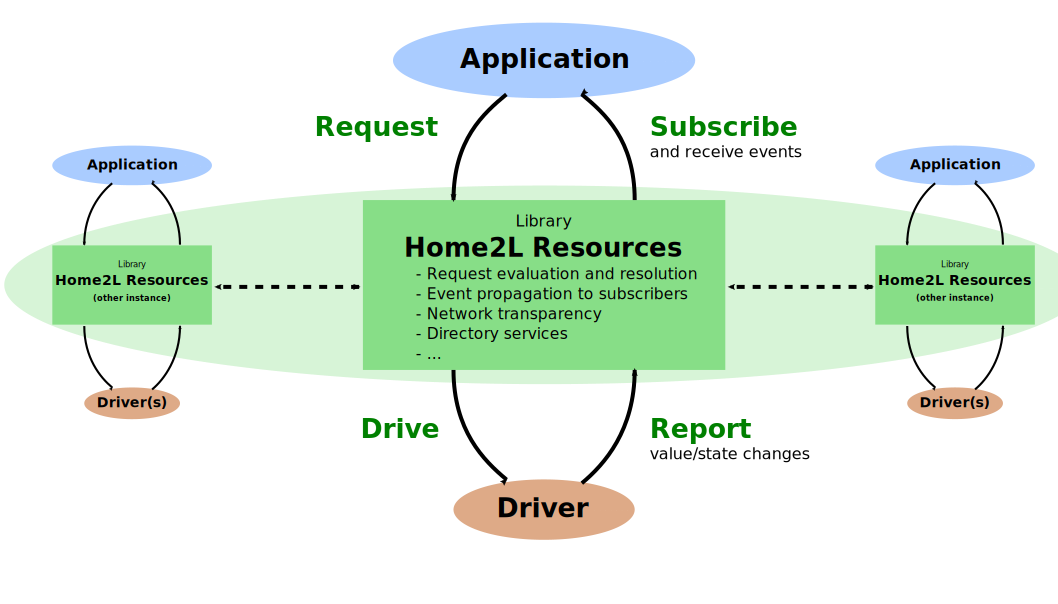
\includegraphics[width=\linewidth,keepaspectratio]{figs/resources-terminology}   %%% eps: inkscape -z -D -T $BASE.svg -E $BASE.eps
  }
  \caption[l]{\emph{Home2L} Resources: Terminology}
  \label{fig:resources-terminology}
\end{figure}

Any application linked against the \emph{Resources} library can provide drivers or
load any of the existing drivers (see Chapter~\ref{ch:drvdev}). This includes
automation rules scripts (see Chapter~\ref{ch:rules}), which may themselves implement
drivers or execute external ones.

In order to ''just'' load driver(s) and export their resources to the cluster,
the tool \toolref{home2l-server} can be used.
This is basically an empty application without any functionality besides operate
the \emph{Resources} library.





%%%%%%%%%%%%%%%%%%%%%%%%%%%%%%%%%%%%%%%%%%%%%%%%%%%%%%%%%%%%%%%%%%%%%%%%%%
\section{Resources, Values and States}
\label{sec:resources-resources}
%%%%%%%%%%%%%%%%%%%%%%%%%%%%%%%%%%%%%%%%%%%%%%%%%%%%%%%%%%%%%%%%%%%%%%%%%%


\subsection{Resources}

A \emph{resource} object has the following attributes:

\begin{itemize}
\item
  a unique resource identifier (URI),
\item
  a typed value and state,
\item
  a ''writeable'' flag,
\item
  a list of listening subscribers,
\item
  a list of pending requests.
\end{itemize}

Resources are organized in a namespace resembling a directory tree with
the following structure:

\begin{lstlisting}
/host/                        ; Host domain: All resources, ordered by host/driver
    <host 1>/
        <driver 1.1>/
            <resource 1.1.1>  ; Resources may be arranged in sub-trees of arbitrary ...
            <resource 1.1.2>  ; ... depth by the driver.
            ...
        <driver 1.2>/
            <resource 1.2.1>
            ...
    <host 2>/
    ...
/alias/                       ; Alias domain: References to resources/subtrees in the host domain
    <alias 1>                 ; Aliases may be arranged in sub-trees and may point ..
    <alias 2>                 ; ... anywhere in the host domain (like symlinks).
    ...
/local/                       ; Alias for /host/<local host>/...
    <driver L.1>
        <resource L.1.2>
        ...
\end{lstlisting}

Except for the \texttt{/local} domain (a shortcut for a process to
access its own resources), any host in the cluster has the same view on
the resource tree.



\subsection{Values}

Resource values are typed, the following types are available:

\begin{enumerate}[a)]

\item Basic types
  \begin{itemize}
    \item \texttt{bool:} Boolean
    \item \texttt{int:} Integer
    \item \texttt{float:} Floating point
    \item \texttt{string:} Text string
  \end{itemize}

\item Special types
  \begin{itemize}
    \item \texttt{trigger:}  Triggerable events (example: \texttt{timer/daily})
    \item \texttt{mutex:} Allows to implement mutual exclusion in a \emph{Home2L} cluster (experimental)
  \end{itemize}

\item Physical (or unit) types
  \begin{itemize}
    \item \texttt{percent ::= <float> \%}
    \item \texttt{temp ::= <float> \textdegree C}
  \end{itemize}

\item Enumeration types
  \begin{itemize}
    \item \texttt{window ::= \{ closed, open, tilted, openOrTilted \}}
  \end{itemize}

\end{enumerate}

The set of unit types and enumeration types may be extended in the future.
The following command prints an up-to-date list of all types for the current installation:

\begin{lstlisting}
home2l shell -e types
\end{lstlisting}



\subsection{States}

A resource can assume one of the following states:

\begin{itemize}
\item
  \texttt{valid:} The value is known and valid.
\item
  \texttt{busy:} The value is known, but the resource is busy.
\item
  \texttt{unknown:} The value is unknown.
\end{itemize}

The \emph{busy} state may indicate that an actor-like resource is
anticipating some new value, but has not yet reached it. For example, if
window shades are requested to close (value 0), the state/value may be
\emph{busy/0} (also written as ''\texttt{~0}'') while the shades are
moving down and then change to \emph{valid/0} when the shades are
actually down. Or, if a computer is requested to start (value \emph{true}),
the driver may report a state/value of \emph{busy/true} while
the machine is booting and then later switch to \emph{valid/true} as soon as
it is ready to use.

The \emph{unknown} state may be reported for a variety of reasons, for example:
\begin{itemize}
\item
  The driver may report it because its device does not deliver valid data.
\item
  The network connection to the serving host was lost.
\item
  The resource does not exist or the host is temporatily down.
\item
  The resource is not subscribed to or not yet initialized.
\end{itemize}

It is important to note that application developers do not have to take
extra actions for error checking. Whenever anything happens that may
make the actual state unsure, the \emph{Resources} library will turn the
state to \emph{unknown} and report this to the subscribers.

The state of a resource is not necessarily the same on all hosts. For example, a resource
may be \emph{valid} on the serving host, but \emph{unknown} on some other host due to
a network problem.





%%%%%%%%%%%%%%%%%%%%%%%%%%%%%%%%%%%%%%%%%%%%%%%%%%%%%%%%%%%%%%%%%%%%%%%%%%
\section{Configuring the Resources Library}
\label{sec:resources-conf}
\toollabel{resources.conf}
%%%%%%%%%%%%%%%%%%%%%%%%%%%%%%%%%%%%%%%%%%%%%%%%%%%%%%%%%%%%%%%%%%%%%%%%%%


The configuration file \toolref{resources.conf} defines hosts,
aliases, and optionally signals for the \emph{Home2L} cluster.

A \emph{host} in this context is a \emph{Home2L instance} running on a
machine. In many cases, if there is only one instance serving resources,
this instance can and should then be identified by its Unix host name in the
etwork and listen on the default \emph{Home2L} port (see below).
If there are multiple serving instances running on the
same machine, listening ports must be assigned manually for all but one
of them.

The default port is defined by the following line:
\begin{lstlisting}
P <port>
\end{lstlisting}

Hosts are declared as follows:
\begin{lstlisting}
H <host ID> [ <hostspec> ]   ; <hostspec> ::= [<instance>@]<net host>[:<port>]
\end{lstlisting}

\verb|<host ID>| is the host ID as visible by other instances.
If no \verb|<hostspec>| is given, \verb|<host ID>| is equivalent to the network host name,
and the default port is used.

\verb|<net host>[:<port>]| is the network host name and port the server is listening on.

\verb|<instance>| is the instance name of the respective server. It is only needed
if multiple servers run on the same machine.

Examples:

\begin{lstlisting}
H eniac   # Single host on machine 'eniac', using the default server port.
H z3-server    server@z3
          # The host ID 'z3-server' refers to 'home2l-server' on machine 'z3',
          # and the server listens on the default port.
H z3-doorman   wallclock@z3:4701
          # The host ID 'z3-doorman' refers to 'home2l-doorman' on machine 'z3',
          # and the server listens on port 4701..
\end{lstlisting}

Servers/hosts are also implicitly declared by the aliases and variables,
which is equivalent to an explicit declaration without \verb|<hostspec>|.

Aliases are defined with the following syntax:

\begin{lstlisting}
A <aliasName> <destPath>
\end{lstlisting}

\verb|<destPath>| may be relativ to \texttt{/host/} or absolute.
Examples:

\begin{lstlisting}
A tempOutside           /host/gatewayhost/weather/tempOutside
A door/backlight        sphinx/gpio/doorBacklight
\end{lstlisting}

These make the current outside temperature (presently delivered via
internet by host \texttt{gatewayhost}) accessible as
\texttt{/alias/tempOutside} and the backlight of the door button as
\texttt{/alias/door/backlight}.

Signals are resources that do not drive any hardware or software, but
simply report back all values driven to them (similar to loopback
devices in Unix). They are useful for intermediate values (for example,
the logical ''and'' of a motion sensor and darkness sensor to indicate
whether a light should be switched on) or for testing purposes (for
example, to temporarily replace a real device by the signal resource,
which can be manipulated manually). They are defined as follows:

\begin{lstlisting}
S <host> <name> <type> [<default value>]
\end{lstlisting}

Signals are handled by the \toolref{home2l-drv-signal} driver, all signals are
read- and writable. Their \emph{URI} is \texttt{/host/<host>/signal/<name>}.
Examples:

\begin{lstlisting}
S turing testBool  bool
S turing testInt   int   7
S turing testFloat float 3.14
\end{lstlisting}


\infobox{
  \textbf{Checklist: Enabling a \emph{Home2L} Server}

  To enable a local server, the following conditions must be met:
  \begin{enumerate}
    \item The application must enable it when calling 'RcInit()' (C/C++) or 'Home2lInit()' (Python).
    \item The configuration option \envref{rc.enableServer} must be 'true'.
    \item It must be declared as a host in \toolref{resources.conf}.
  \end{enumerate}
   Client functionality is always available.
}





%%%%%%%%%%%%%%%%%%%%%%%%%%%%%%%%%%%%%%%%%%%%%%%%%%%%%%%%%%%%%%%%%%%%%%%%%%
\section{Subscriptions}
\label{sec:resources-subscriptions}
%%%%%%%%%%%%%%%%%%%%%%%%%%%%%%%%%%%%%%%%%%%%%%%%%%%%%%%%%%%%%%%%%%%%%%%%%%


Subscriptions are handled by the class \texttt{CRcSubscriber} (see C/C++
API). A subscriber object can subscribe to any number of resources,
eventually selected by wildcards. Resources do not need to exist yet at
the time they are subscribed to.

Subscriber events can be received in multiple ways (see class \texttt{CRcEventProcessor}):

\begin{itemize}
\item
  asynchronously by providing a callback function,
\item
  synchronously and blocking (\texttt{CRcEventProcessor::WaitEvent ()}),
\item
  synchronously and non-blocking (\texttt{CRcEventProcessor::PollEvent ()}).
\end{itemize}

The following types of events may be delivered (see class
\texttt{CRcEvent}):

\begin{itemize}
\item
  \texttt{rceValueStateChanged}: The resource has changed its value.
\item
  \texttt{rceDisconnected}: The connection to the (remote) resource
  has been lost.
\item
  \texttt{rceConnected}: The connection to the (remote) resource has
  been (re-)established.
\end{itemize}

The events \emph{rceDisconnected} and \emph{rceConnected} are relevant,
 if it is important to capture each value/state change and not
just to get the most up-to-date value. These events indicate whether a
gapless event sequence is guaranteed or not.

For those who are missing ''just a normal read'' operation:
As long as a resource is subscribed to by some subsciber, a call to
\texttt{CResource::GetValueState()} and its relatives will always
return the most up-to-date value and state.

With the \refapipython{}, subscribers are used internally if the decorators
\texttt{@onEvent(<resources>)} or \texttt{@onUpdate(<resources>)}
are used. Functions decorated with the former are executed with each
event on one of its resources. The latter is more efficient since it
drops value/state changes if they are already outdated at the time they
are fetched.





%%%%%%%%%%%%%%%%%%%%%%%%%%%%%%%%%%%%%%%%%%%%%%%%%%%%%%%%%%%%%%%%%%%%%%%%%%
\section{Requests}
\label{sec:resources-requests}
%%%%%%%%%%%%%%%%%%%%%%%%%%%%%%%%%%%%%%%%%%%%%%%%%%%%%%%%%%%%%%%%%%%%%%%%%%


In order to properly handle concurrent manipulating accesses to resources, a
\emph{request resolution} mechanism is implemented, which loosely
resembles the concept of \emph{resolution functions} in hardware
description languages (VHDL, Verilog and friends).
Applications never ''write'' to a resource (this would cause serious concurrency
issues), they place \emph{requests}.

Each \emph{request} (class \texttt{CRcRequest}) is associated with a
\textbf{resource}, \textbf{a value} (no state) and a \emph{request identifier (ID)}. The
\textbf{\emph{request ID}} allows to later modify or delete the request from any host.

Additionally, a request may have the following optional attributes:

\begin{description}

\item[\emph{Priority}] (Syntax: \texttt{*<prio>}): The priority of the request.

  This is a number between 0 (= lowest) and 15 (= highest). The default
  priority is 8. If multiple requests at the same priority exist,
  the oldest one dominates. (This behavior is required to
  allow the implementation of Mutexes, where lock owners cannot be
  preempted.)

\item[\emph{Start time} (or \emph{on time})] (Syntax: \texttt{+<time>}): \par
  The request becomes active then, but is not considered before.

\item[\emph{End time} (or \emph{off time})] (Syntax: \texttt{-<time>}): \par
  The request will expire and be discarded after this time.

\item[\emph{Hysteresis}] (Syntax: \texttt{\~{}<hyst>}): Hysteresis time.

  This allows the \emph{Resources} library to postpone the requested action by up to
  \texttt{<hyst>} milliseconds in order to avoid switches forth and
  back again (for example, shutting down a computer that is needed again soon).

  If a positive hysteresis is given, a request will only be activated if
  no change to a different value is planned (according to existing
  requests) within the hysteresis time. Only follow-up events without a
  hysteresis or a hysteresis small enough that they cannot be pushed out
  of the current hysteresis interval are considered.

\end{description}

If no requests are active for a resource, its value will be left
unchanged. It is legal to set the start and end times to identical
values, in which case the value is set once at the specified time (given
that no other request with a higher priority prohibits that) and the
request is deleted again.

Resources of type \texttt{trigger} are processed specially: Only at
the start time, trigger events are generated. Hence, it is
recommended to supply an end time (which may be equal to the start time)
to auto-remove the request.


\infobox{
  \textbf{Examples}

  \begin{enumerate}

  \item
    The user pushes a button to open the window shades. One second later,
    an automatic script decides that the shades should be closed. What should happen now?
    An answer to this question can only be given by the end user. However, the
    \emph{Home2L's} request mechanism allows to implement various different
    solutions.

    Possible solution A:
    \begin{itemize}
      \item The automatic script sets permanent requests \texttt{\#script}
        for a certain value (e.~g.
        0 for ''up'' and 1 for ''down'') and a priority of 5 (the default priority).
      \item Pushing one of the user buttons ''up'' and ''down'' generates a timed requests
        \texttt{\#manual} with the off time attribute set to some time in the future
        (e.~g. 1 hour after the button was pushed)
        and an increased priority of 6. This request will dominate over the script's
        request, and after the off time, the script request will take over again.
    \end{itemize}

    Possible solution B:
    \begin{itemize}
      \item Same as solution A, but with the requests generated with the ''up'' and
        ''down'' button being permanent.
      \item A third push button is used with a ''stop manual mode'' functionality.
        Pushing it removes the \texttt{\#manual} request.
    \end{itemize}

  \item
    A PC-based video recorder can be requested to be on by recording timers as well as
    manually by the user to watch TV. Whenever unused, the PC should shut
    down automatically, but only if the time of the next recording is more
    than 30 minutes in the future to avoid unnecessary power cycles.

    This can be modelled as follows:
    \begin{itemize}
    \item
      The video recorder sets timed requests \texttt{\#timer}
      (with appropriate start and end times) for its recordings with a boolean
      value of '1'.
    \item
      The user sets and deletes untimed manual requests \texttt{\#namual } with
      a value of '1'.
    \item
      To let the computer shut down if not needed, a permanent request
      \texttt{\#default} with a low priority and a value of '0' is set with a
      hysteresis of 30 minutes.
    \end{itemize}

  \end{enumerate}
}




%%%%%%%%%%%%%%%%%%%%%%%%%%%%%%%%%%%%%%%%%%%%%%%%%%%%%%%%%%%%%%%%%%%%%%%%%%
\section{Syntax of Value and Request Specifications}
\label{sec:resources-syntax}
%%%%%%%%%%%%%%%%%%%%%%%%%%%%%%%%%%%%%%%%%%%%%%%%%%%%%%%%%%%%%%%%%%%%%%%%%%


In some places, particularly in the \toolref{home2l-shell} and the \refapipython{},
values, states or requests are printed or accepted in textual form.
This section explains the syntax commonly used for value/state objects and requests.

The syntax of a value/state object is:

\begin{lstlisting}
<valueState> ::= [ "(" <type> ")" ] ( [!]<value>|? ) [ @<time> ]

<value> ::= <bool> | <int> | <float> | <string> | <time> | <unitval> | <enumval>

  <bool>    ::= [0fF] | [1tT+]              : Boolean value
  <int>     ::= [-][0-9]+                   : Integer value
  <float>   ::= [-][0-9]*[.[0-9]+][E[+/-][0-9]+]  : Floating-point value
  <string>  ::= [0-9a-zA-Z\]+ | \0          : String (\-escaped, UTF8 encoding)
  <time>    ::= <time>                      : Time value
  <unitval> ::= [<float>|<int>]<unit>       : Unit value (<unit> is the unit string)
  <enumval> ::= [_a-zA-Z][_a-zA-Z0-9]+      : Enumeration value
\end{lstlisting}

A \texttt{<value>} must not contain any spaces, type and timestamp
attributes are separated by spaces.

Requests are specified as follows:

\begin{lstlisting}
<request> ::= <value> [ <attributes> ]

  <attributes>' is a space-separated subset of:

    #<id>   : Request ID [default: instance name]
    *<prio> : Priority (0..9) [default: 5]
    +<time> : Start time
    -<time> : End time
    ~<hyst> : Hysteresis in milliseconds
\end{lstlisting}

Time values -- either as a value or a an start/end time specification --  can be
specified in several alternative formats:

\begin{lstlisting}
YYYY-MM-DD[-hhmm[ss[.<millis>]]] : Date and time, interpreted as local time

t<unsigned integer>        : Absolute time in milliseconds since the Epoch (POSIX time)

<integer>                  : Relative time, milliseconds from now

hh:mm[:ss[.<millis>]]      : Time relative to 0:00 today; 'hh' may be > 23
                             to specify a time in the coming days
\end{lstlisting}

With the evolution of the \emph{Home2L} software, the information above
may become outdated or incomplete. The most up-to-date information can
be found in the following places of the \refapic{} documentation:

\begin{itemize}
\item
  \texttt{CRcValueState::SetFromStr()} (source file: \texttt{resources/resources.H})
\item
  \texttt{CRcRequest::SetFromStr()} (source file: \texttt{resources/resources.H})
\item
  \texttt{TicksFromString()} (source file: \texttt{common/base.H})
\end{itemize}





%%%%%%%%%%%%%%%%%%%%%%%%%%%%%%%%%%%%%%%%%%%%%%%%%%%%%%%%%%%%%%%%%%%%%%%%%%%%%%%
%
\section{The \emph{Shell} -- The Command Line Interface to \emph{Resources}}
\label{sec:shell} \toollabel{home2l-shell}
%
%%%%%%%%%%%%%%%%%%%%%%%%%%%%%%%%%%%%%%%%%%%%%%%%%%%%%%%%%%%%%%%%%%%%%%%%%%%%%%%


The \emph{Home2L Shell} is a command line interface to the \emph{Resources} library
and can be seen as a ''swiss army knife'' to access and inspect the resources
and servers of a \emph{Home2L} cluster.

With the \emph{Home2L Shell} you can:
\begin{itemize}
  \item list all (server) hosts in the cluster and check their status and availability,
  \item list and inspect the resources directory,
  \item for each resource, see its current value and state, its current list of subscribers and
  all currently active requests,
  \item manually set and delete requests,
  \item monitor resource events,
  \item load and run drivers,
  \item get information on \emph{Home2L} itself (e.g. the list of available value types).
\end{itemize}

The \emph{Home2L Shell} can be run interactively or execute commands in batch mode.
The latter can be used to set/delete requests from a shell script and for logging
of measurements.

Details on the usage of the \emph{Home2L Shell} can be obtained by the 'help' command:
\begin{lstlisting}
$ home2l shell
home2l> help
\end{lstlisting}

Details on the batch usage can be obtained by:
\begin{lstlisting}
$ home2l shell -h
\end{lstlisting}

Section~\ref{sec:tutorial-shell} contains detailed examples for working with the \emph{Home2L Shell}.





%%%%%%%%%%%%%%%%%%%%%%%%%%%%%%%%%%%%%%%%%%%%%%%%%%%%%%%%%%%%%%%%%%%%%%%%%%%
%\section{List of Configuration Parameters}
%\label{sec:shell-env}
%%%%%%%%%%%%%%%%%%%%%%%%%%%%%%%%%%%%%%%%%%%%%%%%%%%%%%%%%%%%%%%%%%%%%%%%%%%
%
%\input{ref_env_shell}





%%%%%%%%%%%%%%%%%%%%%%%%%%%%%%%%%%%%%%%%%%%%%%%%%%%%%%%%%%%%%%%%%%%%%%%%%%
\section{Integrated Drivers}
\label{sec:resources-drivers}
%%%%%%%%%%%%%%%%%%%%%%%%%%%%%%%%%%%%%%%%%%%%%%%%%%%%%%%%%%%%%%%%%%%%%%%%%%



%%%%%%%%%%%%%%%%%%%%%%%%%%%%%%%%%%%%%%%%%%%%%%%%%%%%%%%%%%%%%%%%
\subsection{Driver \emph{Signal}}
\label{sec:drvlib-signal} \toollabel{home2l-drv-signal}
%%%%%%%%%%%%%%%%%%%%%%%%%%%%%%%%%%%%%%%%%%%%%%%%%%%%%%%%%%%%%%%%


The \emph{Signal} driver is always available and allows to declare resources
which just report back any driven value without any technical functionality.

Signals can serve as intermediate resources or for testing purposes.

They can be defined inside a \toolref{resources.conf} configuration file
(see Section~\ref{sec:resources-conf}) or by the API calls
\texttt{RcRegisterSignal()} (C/C++) or \texttt{NewSignal()} (Python).



%%%%%%%%%%%%%%%%%%%%%%%%%%%%%%%%%%%%%%%%%%%%%%%%%%%%%%%%%%%%%%%%
\subsection{Driver \emph{Timer}}
\label{sec:drvlib-timer} \toollabel{home2l-drv-timer}
%%%%%%%%%%%%%%%%%%%%%%%%%%%%%%%%%%%%%%%%%%%%%%%%%%%%%%%%%%%%%%%%


The \emph{Timer} driver provides resources reflecting the current time,
triggers to initiate hourly or daily tasks, and a set of resources
reflecting day and night times, suitable, for example, to control an
automatic outdoor light.

The driver is statically built into the \emph{Resources} library.
It can be disabled using the \envref{rc.timer} setting.



%%%%%%%%%%%%%%%%%%%%%%%%%%%%%%%%%%%%%%%%%%%%%%%%%%%%%%%%%%%%%%%%%
%\subsection{Exported Resources}
%\label{sec:resources-rc}
%%%%%%%%%%%%%%%%%%%%%%%%%%%%%%%%%%%%%%%%%%%%%%%%%%%%%%%%%%%%%%%%%

The \emph{Timer} driver exports the following resources:

\input{ref_rc_resources}





%%%%%%%%%%%%%%%%%%%%%%%%%%%%%%%%%%%%%%%%%%%%%%%%%%%%%%%%%%%%%%%%%%%%%%%%%%
\section{List of Configuration Parameters}
\label{sec:resources-env}
%%%%%%%%%%%%%%%%%%%%%%%%%%%%%%%%%%%%%%%%%%%%%%%%%%%%%%%%%%%%%%%%%%%%%%%%%%

\input{ref_env_resources}





%%%%%%%%%%%%%%%%%%%%%%%%%%%%%%%%%%%%%%%%%%%%%%%%%%%%%%%%%%%%%%%%%%%%%%%%%%%%%%%
%
\chapter{Writing Automation Rules}
\label{ch:rules}
%
%%%%%%%%%%%%%%%%%%%%%%%%%%%%%%%%%%%%%%%%%%%%%%%%%%%%%%%%%%%%%%%%%%%%%%%%%%%%%%%


\section{Overview}
\label{sec:rules-overview}

With the \emph{Home2L} suite, automation scripts are typically written in Python.
Automation scripts are normal Python programs. They can run
on any machine, there can be multiple of them, and they can be started
or stopped any time. The latter is particularly useful for testing and
debugging. Even interactive work in a Python shell is possible.

For a quick start, it is recommended to read the commented sample rules
file also used in the tutorial (Chapter~\ref{ch:tutorial}). Also, it is worth
looking into the implementation of the tutorial's \emph{ShowHouse}, which technically is
implemented in Python like a rules script (see Sections \ref{sec:tutorial-rules} and
\ref{sec:tutorial-goingfurther}.

Typically, a rules script performes a number of initializations, declares a number of
triggered functions, and finally calls \texttt{Home2lRun()}) to enter the main event loop
of the \emph{Home2L} library/package. While the native \emph{Home2L} library makes
use of multi-threading, all Python functions are (and must be)
generally called from the main thread, so that no synchronization measures have
to be implemented in Python code.

The following subsections give some additional hints and references to
the respective places in the \refapipython{}
documentation, which serves as a reference manual for rules writing.



\section{Triggered Functions}
\label{sec:rules-events}


\subsection{Resource Events and Value/State Updates}

Functions to be run can at certain (resource) events can be declared
with the help of the \texttt{@onEvent()} decorator:

\begin{lstlisting}
@onEvent ( <resources> )
def MyFunc (ev, rc, vs):
  # user code
\end{lstlisting}

Functions decorated this way are called for each individual event.
This allows to receive all events without simplificatiopns in the correct
order (important to not miss any event or quick value change) as well
as ''connected'' and ''disconnected'' events.

As arguments, the decorator expects a set of resources, which may be a
single resource or a tuple or list, and each resource may be specified
by a string with its URI or by a reference to the resource object
previously retrieved by \texttt{RcGetResource()}.

The argument \texttt{ev} passed to the user function identifies the type of event,
which can:
\begin{itemize}
  \item \texttt{rceValueStateChanged:} The value or state has changed.
  \item \texttt{rceConnected:} The connection has been (re-)established.
  \item \texttt{rceDisconnected:} The connection has been lost.
\end{itemize}
The arguments \texttt{rc} and \texttt{vs} are the resource and their
current value and state (see class \texttt{CRcValueState}), respectively.

\infobox{
  To avoid race conditions and maintain the precise event model, it is important
  to never query the passed \texttt{rc} for its value/state, but to use the
  passed \texttt{vs} instead.
}



\subsection{Value/State Updates}

Functions decorated with \texttt{@onUpdate()} are called each time
the value or state of a resource changes:

\begin{lstlisting}
@onUpdate ( <resources> )
def MyFunc ():
  # user code
\end{lstlisting}

If the value or state changes very quickly, the user function may be called only for the
latest, most up-to-date value/state. Unlike functions decorated with
\texttt{@onEvent()}, events may automatically be dropped to optimize performance.
This decorator is recommended if it is sufficient to always have the most up-to-date
value/state of a resource, whereas the precise sequence of events is not relevant.
If it is important to not miss any event or quick value change, \texttt{@onEvent()}
should be used.

\infobox{
  \texttt{MyFunc()} has no arguments here. Unlike the precise event model, with the
  ''always up to date'' model assumed here, it is not critical to read the value/state
  of some resource inside the user function. The worst thing that can happen is that
  a value newer than the value that caused the invocation of the user function is
  retrieved.
}



\subsection{Timed Functions}

To run a function a certain time or at certain intervals, the following
decorator can be used:

\begin{lstlisting}
@at ( t = <t>, dt = <interval> )
def MyFunc ():
  # user code
\end{lstlisting}

The \texttt{dt} argument is optional. If unset, the function is called once only.

Sometimes, a timed function is to be run multiple times in different situations.
The reuse of the user function (\texttt{MyFunc()}) is simplified, if

\begin{lstlisting}
RcRunAt (func, t = 0, dt = 0, data = None)
\end{lstlisting}

is used instead of a decorator.



\subsection{Daily Requests}

Often, static requests need to be set that are re-calculated on a daily basis.
For example, an outdoor light might need to be switched on at night depending on the current
sunset and sunrise times. In this case, a \emph{daily rule} my be defined, which
calculates the light-on times at midnight and then sets a request for the light resource
accordingly.

The following decorator defines a function for such daily requests.

\begin{lstlisting}
@daily ( <host set> )
def MyFunc (host):
  ...
\end{lstlisting}

As an argument, the decorator expects a set of host IDs, which is a list or tuple of
strings. The host ID list is used to monitor the availability of the hosts and
eventually also run the user function after a host has crashed or being restarted
and becomes reachable (again).
Besides that, the user function \texttt{MyFunc()} is called with the host ID as an argument on each day, shortly after midnight. It is called once per host, so that it should only
set requests for the host identified by the argument.



\section{Retrieving Resource Values and States}
\label{sec:rules-values}

Due to the highly concurrent nature and implementation of the
\emph{Resources} library, resource values and states may change any
time. To securely retrieve values und states without race conditions,
they must first be captured in a \texttt{CRcValueState} object:

\begin{lstlisting}
vs = rc.ValueState()
\end{lstlisting}

The \texttt{CRcValueState} object \texttt{vs} now contains
information about the type, the value, and the state of the resource.

\infobox{
  To functions decorated with \texttt{@onEvent()}, an appropriately captured value/state
  object is already passed by the \texttt{vs} argument, and that must be used in order
  to avoid race conditions.
}

The value to can then be accessed by:

\begin{lstlisting}
val = vs.Value ()
\end{lstlisting}

If the state of the \texttt{vs} object is 'unknown',
\texttt{Value()} returns \texttt{None}. The caller must consider
this and the code must consistently be written in a way that all calls
of the \texttt{Value()} method can return \texttt{None} any time.

To simplify rules development, the method

\begin{lstlisting}
val = vs.ValidValue(default)
\end{lstlisting}

can be used instead, which alway returns a valid (non-None) value. If the actual value
is invalid, the passed \texttt{default} value is returned.

The following methods may be useful to obtain additional attributes
(refer to the \refapipython{} or \refapic{} documentation for details):

\begin{lstlisting}
Type ()      # the type
State ()     # the state
TimeStamp () # the time stamp
IsValid ()   # True, if the state is 'rcsValid', neither 'rcsBusy' nor 'rcsUnknown'.
IsKnown ()   # True, if the value can be retrieved (state is 'rcsValid' or 'rcsBusy')
\end{lstlisting}

\section{Placing requests}
\label{sec:rules-requests}

Requests can be set or deleted by the following functions:

\begin{lstlisting}
RcSetRequest (resource, reqGid, <args>)
RcSetRequestFromStr (resource, reqDef)
RcDelRequest (resource, reqGid)
\end{lstlisting}

The \texttt{resource} argument can either be a string with the URI or
a reference to the resource object previously retrieved by
\texttt{RcGetResource()}. The \texttt{reqGid} parameter is the
request ID (a string value).

The additional arguments (\texttt{<args>}) contain the value and
optional attributes of the request.

The \texttt{RcSetRequestFromStr()} variant allows to pass all request attributes
by a single string with the same syntax as supported by
\toolref{home2l-shell} and specified in Section~\ref{sec:resources-syntax}.





%%%%%%%%%%%%%%%%%%%%%%%%%%%%%%%%%%%%%%%%%%%%%%%%%%%%%%%%%%%%%%%%%%%%%%%%%%%%%%%
%
\chapter{Writing Drivers}
\label{ch:drvdev}
%
%%%%%%%%%%%%%%%%%%%%%%%%%%%%%%%%%%%%%%%%%%%%%%%%%%%%%%%%%%%%%%%%%%%%%%%%%%%%%%%



%%%%%%%%%%%%%%%%%%%%%%%%%%%%%%%%%%%%%%%%%%%%%%%%%%%%%%%%%%%%%%%%%%%%%%%%%%
\section{Binary Drivers}
\label{sec:drvdev-binary}
%%%%%%%%%%%%%%%%%%%%%%%%%%%%%%%%%%%%%%%%%%%%%%%%%%%%%%%%%%%%%%%%%%%%%%%%%%


\textbf{Examples:} \emph{Demo (\texttt{drivers/demo}), GPIO (\texttt{drivers/gpio})}

Binary drivers are written in native C/C++ code and compiled to a shared
object (\texttt{.so}) file, which at run time can be loaded by a \envref{drv.<id>}
configuration entry.

The driver must contain a single entry function declared as follows:

\begin{lstlisting}
HOME2L_DRIVER(<name>)
(ERcDriverOperation op, CRcDriver *drv, CResource *rc, CRcValueState *vs) {
  switch (op) {
    case rcdOpInit:
      ...
      break;

    case rcdOpStop:
      ...
      break;

    case rcdOpDriveValue:
      ...
      break;
  }
}
\end{lstlisting}

As outlined here, the driver must provide up to three operations:

\begin{description}

\item[The ''Init'' operation]
  registers all resources and initializes the driver itself.

\item[The ''Stop'' operation]
  is called just before the driver gets unloaded. It must stop/join all own background
  threads and shut down its own operations.
  Resources (\texttt{CResource} objects) do \emph{not} have to be unregistered,
  this will be done automatically later.

\item[The ''DriverValue'' operation]
  is only called and required for writable resources. It must drive a new value
  to the real device (e.g.~some actor) to make something happen.
  It is \emph{neither necessary nor allowed} to call any \texttt{CResource} method here.
  The sole task of the driver is to operate its hardware, the driven value with
  a state ''valid'' will be reported automatically.

  If it is not appropriate to report the passed value and a ''valid'' state back this
  time
  (e.g. due to an error or if the actor requires some time to fulfill the requested action),
  the passed \texttt{vs} object should be modified accordingly.

  \infobox{
    For example, a driver for window shades which is requested to close the shades
    would now modify the \texttt{vs} object and set its state to ''busy'' to indicate
    that the shades are now moving down.
    Later, when they are actually closed, the driver calls \texttt{CResource::ReportValue()}
    with a value/state of ''1/valid'' (assuming the value for closed shades is ''1'')
    to report the action was completed successfully.
  }

\end{description}

\textbf{The reporting of values} for sensor-like hardware is typically done
asynchronously. The driver will probably start its own background thread during
initialization which communicates with the hardware. New values for some
resource can be reported any time from any thread by simply calling one
of the \texttt{CResource::ReportValue()} methods (see the \refapic{} for details).





%%%%%%%%%%%%%%%%%%%%%%%%%%%%%%%%%%%%%%%%%%%%%%%%%%%%%%%%%%%%%%%%%%%%%%%%%%
\section{Script-Based Drivers}
\label{sec:drvdev-external}
%%%%%%%%%%%%%%%%%%%%%%%%%%%%%%%%%%%%%%%%%%%%%%%%%%%%%%%%%%%%%%%%%%%%%%%%%%


\textbf{Example:} \emph{Weather (\texttt{drivers/weather})}

A \emph{script-based} driver is typically implemented as a shell script
and communicates with the \emph{Resources} library by its standard input
and output by means of simple text lines. To get an impression of the
simple protocol, one may call such a driver on the command line, for example:

\begin{lstlisting}
$(HOME2L_ROOT)/lib/home2l-drv-weather
\end{lstlisting}

At the script developer's choice, the driver can be operated in one of
two modes:

\begin{enumerate}[a)]

\item
  \emph{Keep-running mode:} The script is running permanently (and
  eventually restarted automatically if it crashes).

\item
  \emph{Polling mode:} The script is run for dedicated operations and
  expected to terminate as soon as these operations are completed.

\end{enumerate}

The script is called by the \emph{Resources} library with the following arguments:

\begin{lstlisting}[language=bash]
<script> -init     # Initialize driver, driver must report its properties (see below)

<script> -restart  # Restart driver (only after abnormal stop in keep-running mode);
                   # The driver does not need to report anything.

<script> -poll     # Driver is polled for new readable values
                   # (only in polling mode)

<script> -drive <resource LID> <value>
                   # Drive a value (only in polling mode);
                   # The driver must report the result by "v" messages.
\end{lstlisting}

In ''keep-running'' mode, values to drive are passed to the script's
standard input as lines with the following format:

\begin{lstlisting}[language=bash]
<resource LID> <value/state>
\end{lstlisting}

The resource's \emph{local ID (LID)} is part of the \emph{URI} following the driver name.
During initialization (\texttt{'-init'} call), the driver is expected
to output a series of lines with the following contents:

\begin{lstlisting}[language=bash]
d <resource LID> <options>  # Declare a resource
p <poll interval>           # Define the polling interval
                            # (0 = no polling; Default = no polling)

.                           # Initialization complete - enter polling mode
:                           # initialization complete - enter "keep running" mode
\end{lstlisting}

The initialization phase must be completed as quickly as possible in the beginning.

In the active phase, lines with the following contents can be written:

\begin{lstlisting}[language=bash]
v <resource LID> <value/state>  # Report a new value/state.
p <poll interval>               # Change the polling interval (polling mode only).
\end{lstlisting}





%%%%%%%%%%%%%%%%%%%%%%%%%%%%%%%%%%%%%%%%%%%%%%%%%%%%%%%%%%%%%%%%%%%%%%%%%%
\section{Python Drivers}
\label{sec:drvdev-python}
%%%%%%%%%%%%%%%%%%%%%%%%%%%%%%%%%%%%%%%%%%%%%%%%%%%%%%%%%%%%%%%%%%%%%%%%%%


\textbf{Example:} \emph{The ShowHouse (\texttt{resources/home2l-showhouse})}

As a third option, drivers can be defined as part of a Python script.

\infobox{
  The demo \toolref{home2l-showhouse} implements a driver for a) a set of (simulated)
  sensors and actors for a virtual building, but also
  b) an asynchronous keyboard driver for its own UI operation.
  The latter demonstrates how to work with background threads.
}

A driver is defined using the decorator

\begin{lstlisting}
@newDriver ( <driver name> )
def DriverFunc (rc, vs):
  ...
\end{lstlisting}

and resources for it are registered by the function

\begin{lstlisting}
RcNewResource (driverName, resourceLID, rcType, writable)
\end{lstlisting}

To improve code readability, \texttt{RcNewResource()} invokations are
allowed before the driver is registered, in which case the resources are
registered later together with the driver. Both drivers and their resources
\emph{must} be registered during the elaboration phase
before calling \texttt{Home2lStart()} or \texttt{Home2lRun()}.

The driver function \texttt{DriverFunc()} is responsible for driving
values to writable resources and is the equivalent to the
\texttt{rcdOpDriveValue} operation in a binary driver (i.e.~must not
do anything else than manipulating its hardware and may eventually
report a failure by changing the state or value of the passed
\texttt{vs} reference.

Value changes (for sensing resources) can be reported by the
\texttt{CResource::ReportValue()} method. With the \refapipython{}, this is
the only method that can be called from any thread. All other API functions
must be called from the main thread.





%%%%%%%%%%%%%%%%%%%%%%%%%%%%%%%%%%%%%%%%%%%%%%%%%%%%%%%%%%%%%%%%%%%%%%%%%%
%
\chapter{Supplied Drivers}
\label{ch:drvlib}
%
%%%%%%%%%%%%%%%%%%%%%%%%%%%%%%%%%%%%%%%%%%%%%%%%%%%%%%%%%%%%%%%%%%%%%%%%%%



%%%%%%%%%%%%%%%%%%%%%%%%%%%%%%%%%%%%%%%%%%%%%%%%%%%%%%%%%%%%%%%%%%%%%%%%%%
\section{Driver \emph{GPIO}}
\label{sec:drvlib-gpio} \toollabel{home2l-drv-gpio}
%%%%%%%%%%%%%%%%%%%%%%%%%%%%%%%%%%%%%%%%%%%%%%%%%%%%%%%%%%%%%%%%%%%%%%%%%%


\subsection{Description}
\label{sec:drvlib-gpio-description}


The \emph{GPIO} driver is a universal driver leveraging the Linux \texttt{sysfs}
GPIO capabilities to access general purpose inputs and outputs (GPIO).

In order to allow GPIOs to be used from a normal user application, they
must be set up properly beforehand.

This preparation requires \texttt{root} privileges and is therefore
done by the \emph{Home2L} init script at boot time.
The names and configurations (e.~g. direction, initial
value) of available GPIOs are defined by symbolic links residing in

\begin{lstlisting}
$HOME2L_ROOT/etc/gpio.<machine name>
\end{lstlisting}

pointing to the actual device, typically:

\begin{lstlisting}
/sys/class/gpio/gpio<n>
\end{lstlisting}

The links are read both by the \emph{GPIO} driver and the init script,
and they must conform to the following naming conventions:

\begin{lstlisting}
$HOME2L_ROOT/etc/gpio.<machine name>/<port name>.<options>

<options> is a sequence of characters and may include:
    i - The port is an input.
    0 - The port is an output with a default value of 0.
    1 - The port is an output with a default value of 1.
    n - The port is active-low (negated).
\end{lstlisting}





%%%%%%%%%%%%%%%%%%%%%%%%%%%%%%%%%%%%%%%%%%%%%%%%%%%%%%%%%%%%%
%\subsection{Configuration Parameters}
%\label{sec:drvlib-gpio-env}
%%%%%%%%%%%%%%%%%%%%%%%%%%%%%%%%%%%%%%%%%%%%%%%%%%%%%%%%%%%%%
%
%
%\input{ref_env_drv_gpio}
%
% ! The configuration may in the future move to 'home2l.conf'.
% ! Then the previous lines have to be commented in.





%%%%%%%%%%%%%%%%%%%%%%%%%%%%%%%%%%%%%%%%%%%%%%%%%%%%%%%%%%%%
\subsection{Exported Resources}
\label{sec:drvlib-gpio-rc}
%%%%%%%%%%%%%%%%%%%%%%%%%%%%%%%%%%%%%%%%%%%%%%%%%%%%%%%%%%%%


The exported resources depend on the configuration (see above).
They are named after their port names (\texttt{gpio/<port name>})
as specified in the name of the symbolic link.





%%%%%%%%%%%%%%%%%%%%%%%%%%%%%%%%%%%%%%%%%%%%%%%%%%%%%%%%%%%%%%%%%%%%%%%%%%
\section{Driver \emph{Weather}}
\label{sec:drvlib-weather} \toollabel{home2l-drv-weather}
%%%%%%%%%%%%%%%%%%%%%%%%%%%%%%%%%%%%%%%%%%%%%%%%%%%%%%%%%%%%%%%%%%%%%%%%%%


\subsection{Description}
\label{sec:drvlib-weather-description}


The \emph{Weather} driver provides local weather information by querying
the \href{http://www.dwd.de/opendata}{Open Data} service of the German Weather
Service (DWD).

\warnbox{
  Other services (e.~g. for weather outside of Germany) are presently
  \emph{not} supported.
}


\subsection{Configuration Parameters}
\label{sec:drvlib-weather-env}

\input{ref_env_drv_weather}


\subsection{Exported Resources}
\label{sec:drvlib-weather-rc}
\input{ref_rc_drv_weather}





%%%%%%%%%%%%%%%%%%%%%%%%%%%%%%%%%%%%%%%%%%%%%%%%%%%%%%%%%%%%%%%%%%%%%%%%%%%%%%%
%
\chapter{\emph{WallClock} -- A Nonobtrusive GUI}
\label{ch:wallclock} \toollabel{home2l-wallclock}
%
%%%%%%%%%%%%%%%%%%%%%%%%%%%%%%%%%%%%%%%%%%%%%%%%%%%%%%%%%%%%%%%%%%%%%%%%%%%%%%%



%%%%%%%%%%%%%%%%%%%%%%%%%%%%%%%%%%%%%%%%%%%%%%%%%%%%%%%%%%%%%%%%%%%%%%%%%%
\section{Overview}
\label{sec:wallclock-overview}
%%%%%%%%%%%%%%%%%%%%%%%%%%%%%%%%%%%%%%%%%%%%%%%%%%%%%%%%%%%%%%%%%%%%%%%%%%


The \emph{WallClock} intends to appear as what the name suggests -- a
wall clock, but with some extra functionality in an unobtrusive way.

The main display (see Figure~\ref{fig:screen-wallclock-home})
shows the time and date, local weather information (if the \toolref{home2l-drv-weather} driver is set
up) and some status about the building (see Section~\ref{sec:tutorial-firststeps-wallclock} for more
explanations).


\begin{figure}[ht]
  \centering
  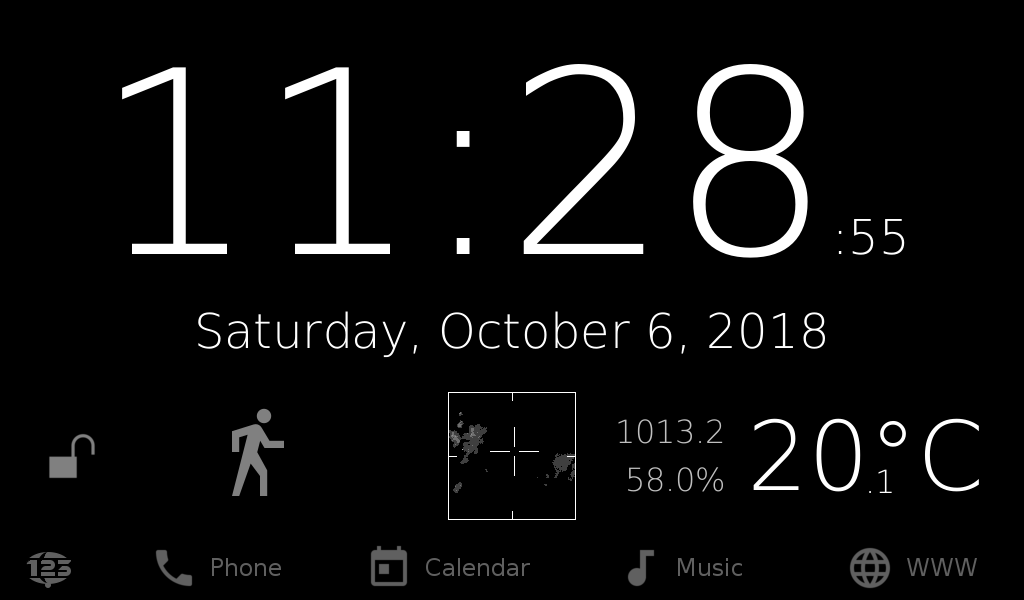
\includegraphics[width=0.7\linewidth]{figs/screen-wallclock-home.png}
  \caption[l]{The \emph{WallClock} Main Screen}
  \label{fig:screen-wallclock-home}
\end{figure}


The following functional modules
(referred to as \emph{applets}), which are frequently useful in a
private household, are integrated in the \emph{WallClock}:

\begin{itemize}
\item
  a SIP-based video phone client (for intercommunication and doorphone funtionality),
\item
  a calendar,
\item
  a music player client (\emph{MPD} client) designed for a distributed
  setup with many rooms and muktiple user in a household,
\item
  an alarm clock to use the \emph{WallClock} device as a radio alarm clock.
\end{itemize}

Ideally, a \emph{WallClock} device is installed in each room in the
house. Due to its resource-aware implementation, low-cost hardware
such as cheap or older second-hand Android tablets should be sufficient.

The \emph{WallClock} is implemented in native code (C/C++) and uses \emph{SDL2} for its UI.
This makes it portable and efficient. So far, the \emph{WallClock} has been tested on
(PC) Linux and on Android, but ports of \emph{SDL2} to many other environments exist
(see \url{libsdl.org}).

\infobox{
  The visualization of the door lock(s) and motion sensor in the lower
  left of the home screen are just a temporary. Future versions will
  contain a generalized solution based on a zoomable floorplan,
  which will be capable of presenting the status of arbitrary gadgets here.
}





%%%%%%%%%%%%%%%%%%%%%%%%%%%%%%%%%%%%%%%%%%%%%%%%%%%%%%%%%%%%%%%%%%%%%%%%%%
\section{The Phone}
\label{sec:wallclock-phone}
%%%%%%%%%%%%%%%%%%%%%%%%%%%%%%%%%%%%%%%%%%%%%%%%%%%%%%%%%%%%%%%%%%%%%%%%%%


The \emph{Phone} applet implements a SIP-based VoIP phone with video
fumctionality and the ability to act as a door phone in conjunction
with \toolref{home2l-doorman}. For example, the applet can offer a door
opener button if its peer is a door phone.

Together with a private branch exchange (PBX) software such as
\emph{Asterisk}, the \emph{WallClocks} can be used as an intercom
system for the house and for a sophisticated door phone system with
multiple door bells and multiple answering stations in the building.

In order to compile the \emph{WallClock} with phone capabilities,
\emph{PJSIP} or \emph{libLinphone} is required.





%%%%%%%%%%%%%%%%%%%%%%%%%%%%%%%%%%%%%%%%%%%%%%%%%%%%%%%%%%%%%%%%%%%%%%%%%%
\section{The Calendar}
\label{sec:wallclock-calendar}
%%%%%%%%%%%%%%%%%%%%%%%%%%%%%%%%%%%%%%%%%%%%%%%%%%%%%%%%%%%%%%%%%%%%%%%%%%


The \emph{Calendar} applet is a graphical calender tool supporting
locally and remotely stored calendars. It supports multiple independent
calendars in a single view, allowing to distinguish private from
business appointments or to manage the activities of multiple family
members.

As its backend and storage format, \texttt{remind(1)} is used.
\texttt{remind(1)} is a mature and powerful command line tool
supporting single events with and without times as well as
many sorts of recurring events. The main advantage is the fact that a
complete calendar is maintained in one \emph{reminders} file with one
event per line. The file is human-readable and can easily be
edited by hand. Synchonization, merging and even
revision control can easily be accomplished by standard tools such as
\texttt{diff(1)}, \texttt{meld(1)} and \texttt{git(1)}.
Several frontends exist for \texttt{remind} (\texttt{tkremind(1)}, for example),
the \emph{WallClock Calendar} is a new one with special support for multiple
calendars.

The calendar files can be stored wherever the user likes -- locally, on
a home server or somewhere else.
For any editing operation, \emph{WallClock Calender} generates a
\texttt{patch(1)} fragment and passes it to a user-configurable script, which
is usually a \texttt{patch} command (see \envref{calendar.cmdPatch}).
The operation for reading a calendar file (usually defined as \texttt{cat <filename>})
is also user-configurable (see \envref{calendar.cmdRead}).

This method for accessing calendar files allows a high degree of flexibility
for where and how they are stored, and the use of \texttt{patch(1)} supports
concurrent editing operations from multiple \emph{WallClock} instances.

To use the \emph{Calendar} applet, the \texttt{remind(1)} command
line tool must be installed on the same computer as the \emph{WallClock}.





%%%%%%%%%%%%%%%%%%%%%%%%%%%%%%%%%%%%%%%%%%%%%%%%%%%%%%%%%%%%%%%%%%%%%%%%%%
\section{The Music Player}
\label{sec:wallclock-music}
%%%%%%%%%%%%%%%%%%%%%%%%%%%%%%%%%%%%%%%%%%%%%%%%%%%%%%%%%%%%%%%%%%%%%%%%%%


The \emph{WallClock Music Player} is a front end for the
\emph{MPD} music player daemon (\url{www.musicpd.org}). It aims to support a home
installations with multiple rooms, multiple users, and multiple virtual or physical
stereo systems. In any room, any user shall be able to control any
stereo system using any \emph{WallClock} device. Everywhere in the house,
he shall have access to the complete music collection and be able to
get it transformed into acoustic air waves by any device he likes:
hifi speakers in the living room, other speakers in the kitchen,
earphones connected to the local device, or bluetooth speakers
coupled with the \emph{WallClock} device. Of course, a user can switch
between them anytime and ''take'' the currently playing music with him as
he moves to another room.

Technically, a ''virtual stereo system'' is an installed \emph{MPD}
instance running on some computer in the household. It has to be
declared in \toolref{home2l.conf} using \envref{music.<MPD>.host}
and related parameters.

If the \emph{MPDs} are configured with an http streaming output, the
music can streamed back and played on the local device (\emph{WallClock}
must be compiled with \emph{GStreamer} support for this).

Figure~\ref{fig:screen-wallclock-music} shows a screenshot
with the usual \emph{MPD} controls on the left and a database and
playlist browser on the right (the title bar can be pushed to navigate
up or switch between the local collection and playlists).


\begin{figure}[ht]
  \centering
  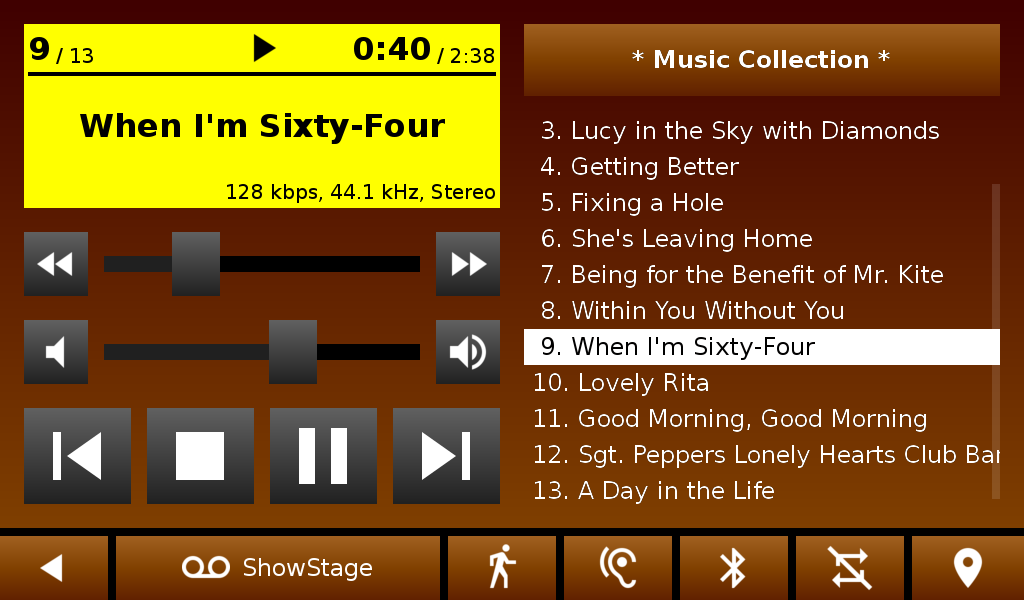
\includegraphics[width=0.7\linewidth]{figs/screen-wallclock-music.png}
  \caption[l]{The \emph{WallClock} Music Player}
  \label{fig:screen-wallclock-music}
\end{figure}


With the buttons in the bottom line you can (from left to right)

\begin{itemize}
\item
  select the ''virtual stereo system'' (\emph{MPD} instance).
\item
  take the currently playing music from one \emph{MPD} instance to another
  (e.g.~to seamlessly continue listening a song when moving from one room to another).
\item
  select the output device (any output configured with \emph{MPD} or
  stream to the local device, if available).
\item
  enable or disable Bluetooth (Android).
\item
  select the repeat mode.
\item
  navigate to the currently playing song.
\end{itemize}

The \rcref{ui/mute} resource allows to mute the music player by automation
rules, for example, if the doorbell rings.

A long push on the ''Music'' launcher on the main screen (Fig.~\ref{fig:screen-wallclock-home})
switches the music player on or off without switching to the music screen.





%%%%%%%%%%%%%%%%%%%%%%%%%%%%%%%%%%%%%%%%%%%%%%%%%%%%%%%%%%%%%%%%%%%%%%%%%%
\section{The Alarm Clock}
\label{sec:wallclock-alarmclock}
%%%%%%%%%%%%%%%%%%%%%%%%%%%%%%%%%%%%%%%%%%%%%%%%%%%%%%%%%%%%%%%%%%%%%%%%%%

The alarm clock can be enabled by pushing the clock display on the main screen.
For each weekday, an individual alarm time can be programmed.

By default, the music player is activated on alarm. If the music player fails
or the music is not loud enough (see \envref{alarm.minLevelDb}), a ringing
sound is played as a fallback.

For the case that the alarm clock fails completely, a dead-man script can
be submitted to another computer, which can then wake you up with some
other means (e.g.~by a wakeup call to your mobile phone).
See \envref{alarm.extAlarmHost}, \envref{alarm.extAlarmCmd} and \envref{alarm.extAlarmDelay}
for details.





%%%%%%%%%%%%%%%%%%%%%%%%%%%%%%%%%%%%%%%%%%%%%%%%%%%%%%%%%%%%%%%%%%%%%%%%%%
\section{List of Configuration Parameters}
\label{sec:wallclock-env}
%%%%%%%%%%%%%%%%%%%%%%%%%%%%%%%%%%%%%%%%%%%%%%%%%%%%%%%%%%%%%%%%%%%%%%%%%%

\input{ref_env_wallclock}


%%%%%%%%%%%%%%%%%%%%%%%%%%%%%%%%%%%%%%%%%%%%%%%%%%%%%%%%%%%%%%%%%%%%%%%%%%
\section{List of Exported Resources}
\label{sec:wallclock-rc}
%%%%%%%%%%%%%%%%%%%%%%%%%%%%%%%%%%%%%%%%%%%%%%%%%%%%%%%%%%%%%%%%%%%%%%%%%%

\input{ref_rc_wallclock}





%%%%%%%%%%%%%%%%%%%%%%%%%%%%%%%%%%%%%%%%%%%%%%%%%%%%%%%%%%%%%%%%%%%%%%%%%%%%%%%
%
\chapter{\emph{DoorMan} -- A Doorbell and Doorphone Service}
\label{ch:doorman} \toollabel{home2l-doorman}
%
%%%%%%%%%%%%%%%%%%%%%%%%%%%%%%%%%%%%%%%%%%%%%%%%%%%%%%%%%%%%%%%%%%%%%%%%%%%%%%%


\section{Overview}
\label{sec:doorman-overview}

\emph{DoorMan} is a doorbell and doorphone service operated on the
command line or as a background service. It must be linked with an IP
phone library (presently \emph{libLinphone}, \emph{PJSIP} support is
planned).





%%%%%%%%%%%%%%%%%%%%%%%%%%%%%%%%%%%%%%%%%%%%%%%%%%%%%%%%%%%%%%%%%%%%%%%%%%
\section{List of Configuration Parameters}
\label{sec:doorman-env}
%%%%%%%%%%%%%%%%%%%%%%%%%%%%%%%%%%%%%%%%%%%%%%%%%%%%%%%%%%%%%%%%%%%%%%%%%%

\input{ref_env_doorman}


%%%%%%%%%%%%%%%%%%%%%%%%%%%%%%%%%%%%%%%%%%%%%%%%%%%%%%%%%%%%%%%%%%%%%%%%%%
\section{List of Exported Resources}
\label{sec:doorman-rc}
%%%%%%%%%%%%%%%%%%%%%%%%%%%%%%%%%%%%%%%%%%%%%%%%%%%%%%%%%%%%%%%%%%%%%%%%%%

\input{ref_rc_doorman}





%%%%%%%%%%%%%%%%%%%%%%%%%%%%% Appendix %%%%%%%%%%%%%%%%%%%%%%%%%%%%%%%%%%%%%%%%


%\appendix


%%%%%%%%%%%%%%%%%%%%%%%%%%%%% Bibliography %%%%%%%%%%%%%%%%%%%%%%%%%%%%%%%%%%%%




%%%%%%%%%%%%%%%%%%%%%%%%%%%%% Index %%%%%%%%%%%%%%%%%%%%%%%%%%%%%%%%%%%%%%%%%%%


\addcontentsline{toc}{chapter}{\indexname}
\printindex


\end{document}
